\chapter{Physical ability metrics} % Main chapter title

\label{ch:phisical_ability_metrics} % Change X to a consecutive number; for referencing this chapter elsewhere, use \ref{ChapterX}


This chapter starts with an an overview of various physical ability metrics for humans and robots, aiming to provide an unifying view of their physical abilities and set the stage for their use in human-robot collaboration scenarios.

The primary focus is put on the polytope-based family of metrics, as one of the well known physical ability metrics for both robots and humans. These metrics enable a unified and accurate representation of their individual abilities. By expressing individual abilities in a unified polytope form, the common physical abilities in collaboration scenarios can be computed using polytope algebra operations, and represented in polytope form as well.

Numerous polytope-based physical ability metrics have been developed in the literature. Therefore, chapter \ref{ch:poly_metrics} presents a comprehensive overview of common polytope-based metrics applicable to both humans and robots. Additionally, chapter \ref{ch:collab_metrics} explores their application in calculating the joint physical abilities of humans and robots when engaged in physical interactions to accomplish specific tasks.

To further enhance the coherence and understanding of different physical ability metrics, chapter \ref{ch:generic_view} also provides a generic polytope algebra-based perspective on these metrics and their categorization them based on their mathematical formulation.

% \todos{
% \begin{itemize}
%     \item This chapter brings the overview of different physical ability metrics for humans, robots and their collaboration
%     \item The chapter further concentrates on polytope based physical ability metrics
%     \item it brings the most common formulations of different polytope based metrics for humans and robots
%     \item it shows how these metrics can be used to characterise the joint abilities in case of physical human robot interaction
%     \item finally it brings a generic polytope algebra based view on different polytope base physical ability metrics and their categorisation with respect to their formulation
% \end{itemize}
% }

\section{Common physical ability metrics}
% \todos{
% \begin{itemize}
%     \item Physical ability metrics are defined as mapping of the actuation space limits of robots and humans to the cartesian / task space 
%     \item many different metrics in the literature
%     \end{itemize}
% }

Physical ability metrics describe how different limitations of robotic system's actuators and mechanics, as well as different biomechanical and biological limitations of human bodies, influence their respective capacity to execute movements, generate forces, achieve different precision levels or produce other physical values necessary to execute a certain task.

They are important tools for analysis and design of robotic manipulators as well as for defining the tasks they are capable of executing. In case of humans, they are used to ensure human safety by studying the ergonomics of different tasks and workspaces. Finally, they have a great potential to be used in human-robot collaboration scenarios to characterise joint physical abilities of robots and humans, with the aim to improve the quality, performance and safety of their physical interaction.

However, not all the physical ability metrics are made equal. Therefore, this chapter brings an overview of different physical ability metrics for robots and humans and discusses their potential use for human-robot collaboration.

\subsection{Metrics in robotics}
In robotics, physical ability metrics metrics are used as performance metrics, establishing the relationship between the robot's actuator limit (joint positions $\bm{q}$, velocities $\dot{\bm{q}}$, torques $\bm{\tau}$, etc.) and the achievable sets of different task related physical values, such as achievable positions $\bm{x}$, velocities $\dot{\bm{x}}$, external wrenches $\bm{f}$ and similar. The physical ability metrics are usually divided in two groups with respect to their scope: \textit{Global} and \textit{Local} metrics  \cite{russo2022measuring}. 

Global metrics present robot state independent metrics evaluated by taking in consideration all the possible robot states. Examples of such metrics are robot's reachable workspace \cite{Zacharias2007,Vahrenkamp2016,kucuk2005robot}, a set of cartesian positions the robot can reach given the limitations of its actuator positions, or its wrench closure workspace \cite{gouttefarde2006determination,Lau2011}, a set of cartesian positions robot can reach while guaranteeing the ability to apply certain set of wrenches. Additionally, a different set of global metrics is based on finding the \textit{worst-case} scenario values of physical ability metrics within the workspace, and used to guarantee certain physical ability values for a given robot. Such metrics are robot's payload, its \textit{worst-case} carrying capacity usually expressed in kilograms, robot's \textit{worst-case} positioning accuracy or positioning repeatability \cite{russo2022measuring}. Global metrics are computationally expensive as their evaluation requires sweeping through all the robot states, however they are typically calculated only once for particular robot design or given task.
%\todo{underestimation}
One traditional application for such performance metrics is robot design, as they enable verifying and guaranteeing that the robotic system, being designed, is compliant with all the requirements of the tasks. 

Local metrics, on the other hand, are robot state dependant performance metrics which can be evaluated relatively efficiently for any given robot state. In that way they are capable of characterising the influence of both robot actuator limits and robot state on the task related variables. Therefore, as opposed to the global metrics, they enable comparing the performance of, not just different robots, but also different states of the same robot with respect to the task. The local physical ability metrics are often represented as scalar values indexes for a given robot's state \cite{Patel2015}. Some of the most well known ones are: manipulability index \cite{yoshikawa_manipulability_1985} and condition number \cite{Gosselin1991} which characterise the movement and dexterity capacity of the robot as well as its accuracy \cite{merlet_jacobian_2006}, dynamic manipulability \cite{yoshikawa1985dynamic} that characterises the task related acceleration capacity or the robot stiffness \cite{PASHKEVICH2011662} characterising the robot's tasks related load and deflection relationship.
Having a scalar metric is beneficial when it comes their use in different optimisation scenarios, for example in robot design refinement \cite{kucuk2005robot} or in robot trajectory generation \cite{Guilamo2006}. 

However having scalar representation of robot's capabilities can be constraining in certain applications, especially if the task has more than one dimension, for example movement in the 3d space. Different local performance metrics have been developed over years, especially based on ellipsoid metrics, that are capable of characterising the robot's task related capacity in multi-dimensional task space. Ellipsoid metrics describe the ease of generating different task related variables (velocity, acceleration, inertia, stiffness etc.) in different directions of task space. One such metric, called manipulability ellipsoid, developed by Yoshikawa \cite{yoshikawa_manipulability_1985}, describes the capacity of robotic system to generate task space velocities and can be described mathematically as
\begin{equation}
    \mathcal{E}(\bm{q}) = \left\{ \dot{\bm{x}} ~|~ \dot{\bm{x}} = J(\bm{q})\dot{\bm{q}},~~ ||\dot{\bm{q}}||_2 \leq 1 \right\}
\end{equation}
where $J(\bm{q})$ is robot's state $\bm{q}$ dependant jacobian matrix relating its joint velocity $\dot{\bm{q}}$ and the task space velocity $\dot{\bm{x}}$. This metric evaluates the capacity of generating different task space velocities $\dot{\bm{x}}$ by considering that the robot can generate all the joint velocities $\dot{\bm{q}}$ with equal ease, represented by the condition $||\dot{\bm{q}}||_2 \leq 1$. Similar ellipsoid based metrics can be used to characterise the force capacity of robotic systems \cite{chiacchio_global_1991}, acceleration capacity \cite{yoshikawa1985dynamic}, inertia \cite{Asada1984}, stiffness \cite{ajoudani2015role}, etc. 
%\todo{few applications, say they are efficient to calculate}

The hypothesis, the ellipsoid based metrics make, of equal capacity (ease of generating motion, forces, accelerations etc.) all the robot joints, in general case, does not reflect the true nature of robot actuation capacity. Robots have different actuators for different joints that can have substantially different characteristics. Therefore, in order to evaluate more accurate robot's task space capacity (motion, force, acceleration etc.) their true limits have to be taken in consideration. The ellipsoid metrics can be extended to take in consideration non-uniform robot actuation limits, by introducing scaling
\begin{equation}
    ||W\dot{\bm{q}}||_2 \leq 1, \quad W=\text{diag}\left(\left[\dot{q}_{1,max} ,~\dot{q}_{2,max} , ~\ldots\right]\right)^{-1}
    \label{eq:scaled_norm}
\end{equation}    
where scaling matrix $W$ normalises the robot joint velocity capacity. However, they still make the assumption that the limits can be represented in the euclidean norm  $||.||_2$ form, which in general case is not true \cite{Lee1997manip}. As the real robot limits are usually expressed in a form of ranges $ \dot{\bm{q}}_{min} \leq \dot{\bm{q}} \leq \dot{\bm{q}}_{max}$, the euclidean norm (\ref{eq:scaled_norm}) based representation is an underestimation of the true robot's capacities. This effect is shown on the example of manipulability ellipsoid metric on Figure \ref{fig:ellip_poly_dif}. 

\begin{figure}
    \centering
    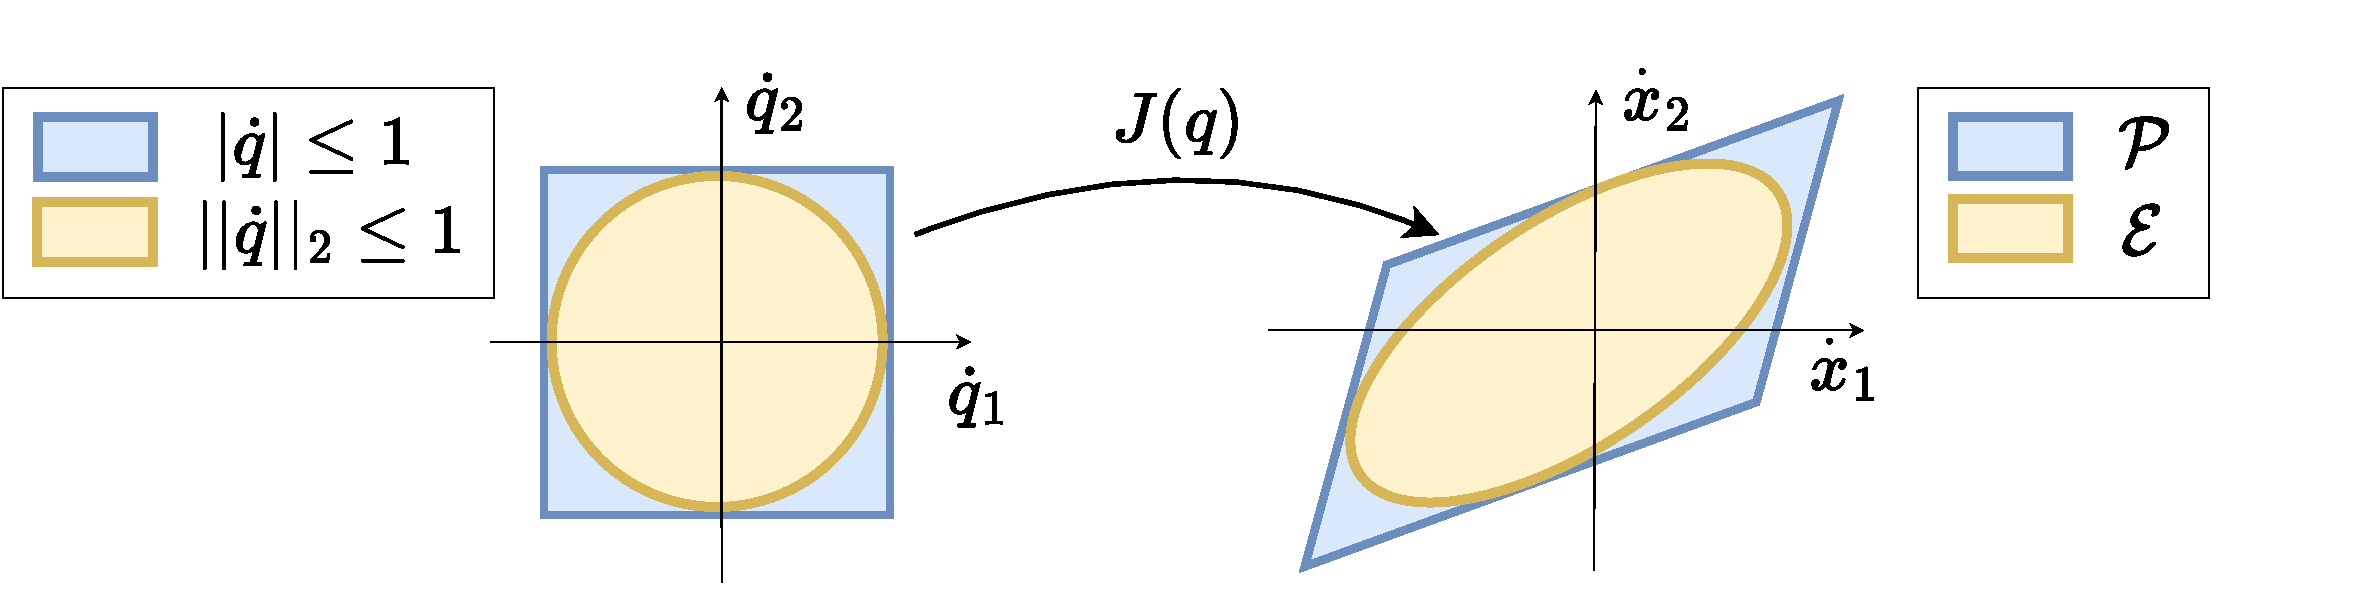
\includegraphics[width=0.7\textwidth]{Chapters/imgs/ellip_poly.pdf}
    \caption{An example manipulability polytope and ellipsoid geometry for a planar $m=2$ robot with $n=2$. The difference between the joint space limits for ellipsoid described with $||\dot{\bm{q}}||_2\leq1$ (orange) and the range limits $\bm{-1}\leq\dot{\bm{q}}\leq\bm{1}$ (blue) is shown on the right. The difference in obtained achievable task space velocity $\dot{\bm{x}}$ polytope $\mathcal{P}$ (blue) and ellipsoid $\mathcal{E}$ (orange) is shown on the right plot. The plot show that both in joint and task space the ellipsoid metric is an underestimation of the true robot's capacity.}
    \label{fig:ellip_poly_dif}
\end{figure}

A family of local performance metrics that is capable of considering the true robotic actuator limits is a family of metrics based on convex polytopes. As opposed to the manipulability ellipsoid $\mathcal{E}$, manipulability polytope can be defined as
\begin{equation}
    \mathcal{P}(\bm{q}) = \left\{ \dot{\bm{x}} ~|~ \dot{\bm{x}} = J(\bm{q})\dot{\bm{q}},~~ \dot{\bm{q}}_{min}\leq\dot{\bm{q}} \leq \dot{\bm{q}}_{max} \right\}
\end{equation}
Manipulability polytope $\mathcal{P}$ represents an exact solution of the robot's task space velocity capacity, given robot's state $\bm{q}$
and its joint velocity limits $\dot{\bm{q}}$. The difference between the manipulability ellipsoid $\mathcal{E}$ and polytope $\mathcal{P}$ is shown for a simple 2d example on Figure \ref{fig:ellip_poly_dif}.
Polytope based physical ability metrics are the most complete local representation of task space physical abilities of robotic systems and they are used to characterise many task related physical values such as velocities \cite{Lee1997manip, long_constrained_2020}, forces \cite{chiacchio_evaluation_1996}, accelerations \cite{chiacchio_2000}, stiffness \cite{ajoudani2015role}, positioning accuracy \cite{pholsiri2005real}, etc.
The main downside to the polytope based metrics with respect to the ellipsoid based metrics is their computational complexity, making their use somewhat limited to non time critical applications.
% \todos{say that most of the stuff done with other metrics can be done with polytopes as well}

% \todos{
% \begin{itemize}
%     \item for robotics
%     \begin{itemize}
%         \item used to evaluate the robot capacity to execute certain tasks
%         \item to design more capable robots
%         \begin{itemize}
%             \item different visual metrics cable of being used to guarantee stuff
%             \item usually calculated in advance for the whole robot workspace 
%             \item payload for example, or reachable workspace, or wrench closure workspace for parallel robots
%             \item typically not taking in consideration robot's dynamics
%         \end{itemize}
%         \item to exploit robot's full potential when controlling it (or planning its movements)
%         \begin{itemize}
%             \item used in optimisation
%             \item different scalar metrics that are easy to calculate in real time
%             \item manipulability index, and all the other indexes from the overview paper
%             \item also ellipsoids were used for this to find the directions with max movement capacity
%         \end{itemize}        
%     \end{itemize}        
% \end{itemize}
% }

\subsection{Metrics for humans}

Evaluating physical abilities of humans is a much more challenging than for robotic systems, as human bodies are much more complicated systems that depend of both on biological and biomechanical, as well as cognitive and psychological factors.

Measuring different physical abilities of human subjects is traditionally done experimentally. The ability of human subjects to generate different physical values such as forces \cite{HODDER2016Testing,HOLZBAUR20072442}, movements \cite{Jessop2016} or stiffnesses \cite{Tsuji1995,Artemiadis2010}, is tested in laboratory environment for a set of predefined human postures or movements. These experiments enable finding precise physical abilities of one or multiple subjects, for the tested motions and postures.  Such experimental analysis are common tools for evaluation of physical abilities in sports \cite{Jessop2016}, where the motions and postures of interest are usually well define, and in rehabilitation \cite{HAISMA2006741} where the aim is to measure the progress of the human subject's recovery. However due to the large variability in human bodies and movements, it is challenging to generalise these results to the human subjects who were not part of the experiments, as well as to different postures and movements, of the same human subjects, that were not tested in the experiments.

In more varied and unstructured settings, where the human postures and movements are harder to characterise, such as in factory setting, the experimental metrics are impractical. For these scenarios, instead of characterising the physical ability of human subject directly, different metrics are developed aiming to evaluate the ergonomics of human postures and movements when executing tasks. These metrics are able to account for variations in human body anthropomorphic structure as well as for different movement and forces generation requirements of the tasks. Such metrics are often defined in a form of standards, such as \textit{Rapid Entire Body Assessment} (REBA) \cite{reba}, \textit{Rapid Upper Limb Assessment} (RULA) \cite{rula} or DULA and DEBA \cite{Yazdani2022} ( their differentiable equivalents), and manuals, such as Great Britain's \textit{Manual Handling Operation Regulations} \cite{health1992manual} or NASA's \textit{Man-systems integration standards} \cite{nasa}. These metrics are designed to give a certain score or a recommendation for the human postures, movements or force generation requirements of the task, in order to evaluate if the task is well suited for human's physical abilities. Common applications of these metrics, in factory settings, have for a goal to evaluate and improve the ergonomics of human's tasks \cite{Busch2017} and workplace layouts\cite{ORE20161, Lietaert2019}. However, these metrics, in order to be task and human subject agnostic, make coarse approximations of human physical abilities which are constraining when it comes to the online human robot collaboration scenarios. 
%\todo{motivate better, a sentence about problems} 

In order to characterise human's physical abilities, more finely, without the need for time consuming and impractical experimental evaluation, different metrics based on human musculoskeletal models are proposed. Human musculoskeletal models are relatively complete models of human bodies capable of describing different human body's biological and biomechanical parameters as well as its rigid body dynamics. Musculoskeletal models are actuated by the muscle-tendon units, capable of applying a range of contracting forces, accelerations and velocities. Similar to the robotic systems, several global and local physical ability metrics, based on musculoskeletal models, can be calculated by evaluating how different limits of the muscles as actuators effect the human's task related physical abilities, such as to generate forces or motions. 

Several global physical ability metrics based on musculoskeletal models are introduced in literature, such as human upper extremity reachable workspace \cite{Lenarcic1994,Kurillo2013} or comfortable reachable workspace \cite{Figueredo2021}, the comfortablility map of the reachable workspace of human's upper limbs evaluated using RULA and REBA ergonomics scores. In addition to the global metrics many robotics inspired local, state dependent, metrics have been developed as well. Different authors have used ellipsoid based metrics to asses the velocity (manipulability) \cite{Rezzoug2012manipulability}, force \cite{rezzoug_application_2012, lazinica_higher_2010}, acceleration \cite{khatib2009robotics} and stiffness \cite{Artemiadis2010} capacity of humans based on their musculoskeletal models. Several of these metrics have been extend to the more complete polytope representation as well, such as force polytope \cite{sasaki2011vertex, rezzoug_application_2012, carmichael_estimating_2013} and acceleration capacity polytope \cite{khatib2009robotics, demircan2012muscle}. As in the case of robotic systems, polytope based metrics present the exact solution to the physical ability evaluation, given an appropriate musculoskeletal model. However, as the musculoskeleral models are only an approximation of the true physics of human bodies the accuracy of calculated physical ability metrics relies entirely on the correspondence between the model and the human subject. Multiple experimental studies were conducted on for the human upper limb force generation capacity, by Rezzoug et al. \cite{biomechanics1010008}, Hernandez et. al \cite{HERNANDEZ2015} as well as Sasaki et al. \cite{lazinica_higher_2010}, where the experimental results were compared to the force capacity polytope and ellipsoid metrics. Their results confirm that the polytope metrics correspond better to the experimentally obtained capacity of the human subjects. However, the results further underline the importance of having an appropriate musculoskeletal model of the human subject. Even though many strategies have been developed for fitting the musculoskeletal models to human subjects in the biomechanics literature moslty based on different forms of scaling \cite{Lund2015, Ziyun2019}, it is still an open field of research. 

With the assumption of an appropriate and well adapted human musculoskeletal model of the human subject, the polytope and ellipsoid based metrics present an accurate estimation of the human's task related physical abilities. 
Even though polytope metrics are more accurate estimation, ellipsoid based metrics, due to their computational efficiency, are still a preferred choice when it comes to evaluating human's physical ability metrics, especially in real time applications. The difference in computational complexity between polytope and ellipsoid evaluation for musculoskeletal models is even more exaggerated than for the robotic systems. As the musculoskeletal models often have many muscles (often more than 50) final polytope geometry becomes complex which ultimately has a negative impact of their execution time.

% \todos{
% \begin{itemize}
%     \item for humans
%     \begin{itemize}
%         \item for humans the metrics are mush less exact, mostly empirical
%         \begin{itemize}
%             \item in labs
%             \item per subject
%             \item hard to generalize
%             \item takes time
%         \end{itemize}
%         \item simpler metrics 
%         \item used to evaluate the ergonomics of the human posture, his task or his workspace
%         \begin{itemize}
%             \item evaluated in-situ
%             \item different score based scalar metrics
%             \item ergonomics scores based on different metrics and manuals
%             \item rula, reba, payload manual, nasa and similar
%         \end{itemize}        
%         \item different set of metrics based on human miscalculate models
%         \item based on exact evaluation of different metrics (similar to robots)
%         \begin{itemize}
%             \item used to evaluate maximal human capacities
%             \item more or less all the metrics as for robots can be used
%             \item ellipsoids and polytopes to evaluate the maximal force capacity
%         \end{itemize}   
%         \item there are also those who try to combine the two
%         \item standards + musculoskeletal stuff
%         \begin{itemize}
%             \item comfortability metrics ( a combination of the two ) \cite{Figueredo2021}
%             \item however calculated in advance and relatively complicated to use, no dynamics
%         \end{itemize}   
%     \end{itemize}
    
% \end{itemize}
% }

\subsection{Collaborative metrics}

Human's and robot's individual physical ability metrics have been used in different human-robot collaboration scenarios. Robot's physical abilities are often calculated in order to make sure that the task requirements comply with robot's capacity, while human's physical ability and ergonomics metrics are then used to design the suitable robot behavior in order to make the human's task and posture more ergonomic. Such collaboration strategies consider the robot to the the action vector with limited resources whose job is to improve the task performance and the human ergonomics at the same time. Examples of such human-centered collaborative scenarios are described by Kim et al. \cite{KIM2021102084}, Carmichael et al. \cite{carmichael2013admittance,carmichael_towards_2011} and Pertic et al. \cite{petric2019assistive}.

However, when it comes to the human-robot collaboration scenarios where a human and a robot interact physically in order to execute a certain task, characterising their joint physical abilities is still an open research question. Human and robot physical abilities are often expressed in different ways, with different units and with fundamentally different metrics, making the procedure of combining them challenging. Therefore, in order to characterise their joint physical capacity, the first step is to express their individual physical abilities need in the same unifying form. 

When it comes to multi-robot physical collaboration, Chiachio et al. \cite{chiacchio_global_1991} have shown that ellipsoid based metrics can be used to calculate their combined joint velocity (manipulability) capacity. The final joint capacity has an ellipsoid form as well.  However, in their formulation, the collaboration of multiple robots is essentially seen as one larger robot, combining all the joints of all the robots, resulting in the robot with $n=n_1 + n_2 + \ldots$ degrees of freedom.
\begin{equation}
    \bm{q} = \begin{bmatrix}
        \bm{q}_1\\ \bm{q}_2 \\ \ldots
    \end{bmatrix}, \quad
    \dot{\bm{q}} = \begin{bmatrix}
        \dot{\bm{q}}_1\\\dot{\bm{q}}_2 \\ \ldots
    \end{bmatrix}, \quad
    J(\bm{q}) = \text{diag}([J_1(\bm{q}_1),~ J_2(\bm{q}_2),~\ldots])
\end{equation} 

\begin{figure}[!h]
    \centering
    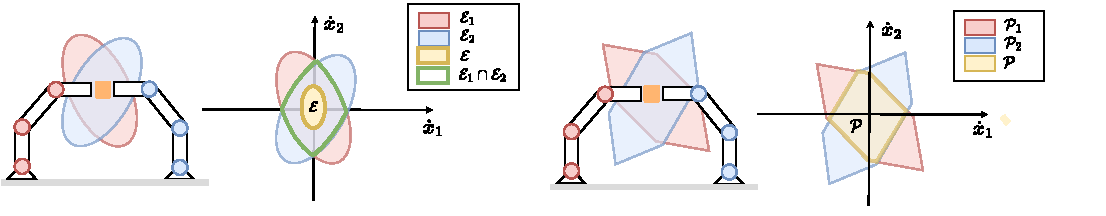
\includegraphics[width=1.05\linewidth]{Chapters/imgs/collab_manip_poly.pdf}
    \caption{Comparison of using polytopes (right) and ellipsoids (left) for collaborative physical ability calculation. Using polytopes, the common velocity capacity of the two robots is calculated as the intersection of their polytopes $\mathcal{P}=\mathcal{P}_1 \cap \mathcal{P}_2$. In ellipsoid case the intersection of the ellipsoids (green) is no longer an ellipsoid and it is hard to characterise, while the collaborative ellipsoid $\mathcal{E}$ (orange) introduced by Chiachio et al. \cite{chiacchio_global_1991} is a large underestimation of the true joint capacity.}
    \label{fig:collab_mani_poly}
\end{figure}
With such large number of joints, the euclidean norm $||.||_2$ limits present a large under-approximation of the real robot's limits, resulting in large under-approximation of the true capacity of the collaboration. As shown on the example on Figure \ref{fig:collab_mani_poly}, a more precise approach would be to intersect the ellipsoids calculated independently for all the robots $$\mathcal{E}=\mathcal{E}_1 \cap \mathcal{E}_2  \cap \ldots$$ However, the intersection operation over ellipsoids is hard to characterise and to evaluate and even if the intersection of the ellipsoids is obtained, it is just an approximation of true common capacity. 

Expressing the robot's physical ability in the polytope form however is not just the exact solution, but enables using the polytope algebra to do different operations, such as sum, intersection and union. These operations are well defined and can be calculated efficiently. The work from Jihong Lee \cite{lee2001velocity} shows that polytopes metrics can be used to describe the common velocity capacity of multi-arm collaborative robotic system.  The work describes an efficient way of calculating the joint velocity capacity by intersecting the individual polytopes of each one of the robots involved, resulting in a convex polytope shaped joint velocity capacity $$\mathcal{P}=\mathcal{P}_1 \cap \mathcal{P}_2  \cap \ldots$$
By exploiting different polytope algebra operations it is possible to express different physical collaboration scenarios as well. For example, if now the robots would be re-arranged from the parallel to the serial configuration, where the robot would be stacked one on top of the other, their joint velocity capacity would correspond to the minkowski sum of their individual capacity $$\mathcal{P}=\mathcal{P}_1 \oplus \mathcal{P}_2  \oplus \ldots$$

\begin{figure}[!h]
    \centering
    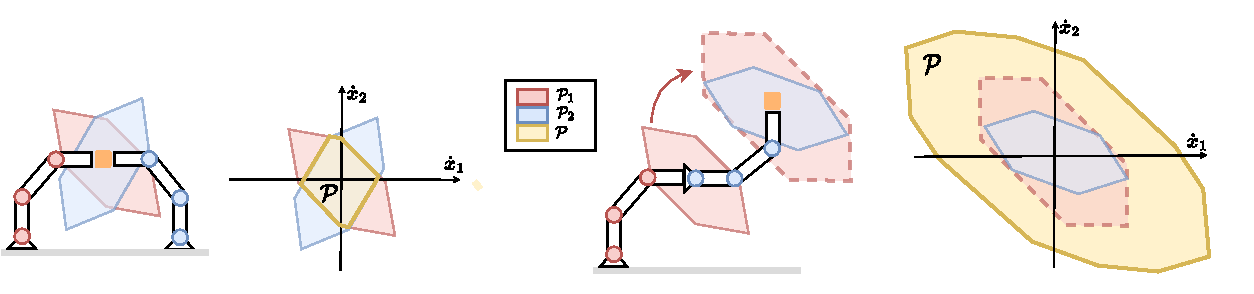
\includegraphics[width=\linewidth]{Chapters/imgs/collab_serial_parallel.pdf}
    \caption{Two examples of using polytope based metrics for joint achievable velocity capacity calculation of multiple robots collaborating. Figure on the left shows the parallel collaboration where the common capacity is calculated with the intersection, and on the right serial collaboration where the common capacity is a minkowski sum of their individual capacity.}
    \label{fig:collab_serial_parallel}
\end{figure}
Figure \ref{fig:collab_serial_parallel} shows a simplified plannar example of the joint velocity capacity calculation for parallel and serial robot arrangement.

Finally, as many different physical ability metrics can be expressed in polytope form, for both robots and humans, combining the individual polytopes using the polytope algebra opens many doors for characterising their common physical abilities in different physical collaboration scenarios. 

% \todos{
% \begin{itemize}
%     \item what about collaboration metrics
%     \item Some metrics have been used but still very limited
%     \item when it comes to characterising their common capacity
%     \begin{itemize}
%         \item payload metrics might be used - very limiting
%         \item and ellipsoid based stuff from chiacchio - robots
%         \item lee also with polytopes a bit - robots
%         \item we still lack proper metrics to unify the humans and robots
%         \item they are usually expressed in different ways and hard to combine
%     \end{itemize}
%     \item Different ways of enhancing collaboration using physical ability metrics
%     \begin{itemize}
%         \item Collaborative workspace design for example - vincent paper
%         \item visualisation to the user 
%         \item Communicate the current robot state to the operator when collaborating
%         \item assist as needed control of exoskeletons also maybe (ellipsoids petric + polytopes carmichael)
%         \item but still not considering robot's capacity - robot only adapts to the human needs
%     \end{itemize}
% \end{itemize}
% }


\subsection{Why polytopes?}

As described in previous chapters, polytope based physical ability metrics represent the exact solution for expressing the abilities of robotic manipulators, as well as the most complete approximation of human physical abilities based on musculoskeletal models. Additionally, since most of the well known polytope metrics for robotic systems can be formulated as polytopes for musculoskeletal models as well, they enable evaluating and comparing human's and robot's physical abilities in a unified manner. Finally, the polytope algebra enables operations over multiple polytopes and in that way enables characterising joint physical abilities of humans and robots involved in different physical collaboration scenarios. 

Having a metric with the convex polytope form has several other benefits as well. Polytopes can be represented as a set of vertices, that can be easily triangulated and visualised as a triangulated mesh. Most of the standard visualisation tools can visualise triangulated meshes in very efficient manner, even in real time.
Polytopes can be expressed as a set of linear inequalities $A\bm{x}\leq\bm{b}$, that can be integrated in different optimisation problems in a form of linear inequality constraints. Inequality constraints can be easily integrated with most of standard quadratic (QP) 
\cite{boggs_tolle_1995} and linear (LP) program \cite{GOLDFARB198973} solvers.

% \todo{many algos in literature}

However, the computational cost of evaluating polytopes is much higher than other local metrics, such as ellipsoids, which makes their use in time-critical applications still relatively less common, especially for human physical ability evaluation due to the added complexity of musculoskeletal models. 



% \todos{
% \begin{itemize}
%     \item polytope based metrics might be able to close the gap
%     \item in our opinion the best ones - unifying most of the other metrics
%     \item exact solution 
%     \item encapsulate many of the other metrics inside (volume, direction of maximal magnitude, singularity, ....)
%     \item can be easily visualised
%     \item defined both for robots and humans (based on musculoskeletal models)
%     \item can be used in optimisation
%     \item operation over polytopes (sum, intersection union) well defined as opposed to the other metrics
% \end{itemize}
% }
\section{Polytope based physical ability metrics}
\label{ch:poly_metrics}
Polytope based physical ability metrics are numerous in literature, therefore the aim of this chapter is to provide a non-exhaustive overview of common polytope based physical ability metrics for robotic systems and humans, based on their musculoskeletal models. Additionally, Chapter \ref{ch:collab_metrics} demonstrates the use of these metrics to calculate the physical abilities in collaborative scenarios. Finally, Chapter \ref{ch:which_metric_which} brings the categorisation of the common polytope based metrics and with respect to the nature of their formulation.

\subsection{Robotic manipulators}
\label{ch:robot_metrics}

Physical ability metrics based on polytopes are most complete local, state dependent, metrics for the performance analysis of robotic systems \cite{pholsiri2005real,Finotello1998}. They describe a mapping between the robot's actuator limits (torques $\bm{\tau}$, accelerations $\ddot{\bm{q}}$, velocities $\dot{\bm{q}}$, etc.) and the limits of different task space variables (wrenches $\bm{f}$, accelerations $\ddot{\bm{x}}$, velocities $\dot{\bm{x}}$, etc.) . 

The aim of this chapter is to provide an overview of common polytope based physical ability metrics for robotic systems in an unified view.  Therefore, chapter \ref{ch:robot_dyn_kin} beings a quick overview of the dynamics and kinematics equations for robotic systems, used for different metrics definitions. Definitions 
of common polytope based physical ability metrics are then described in subsequent chapters.

\subsubsection{Dynamics and kinematics relationships}
\label{ch:robot_dyn_kin}
The actuation limits, of a robotic manipulator with $n$ joints, are commonly specified as independent ranges of achievable actuator positions $\bm{q}\in \mathbb{R}^n$, velocities $\dot{\bm{q}}\in \mathbb{R}^n$, actuator torques $\bm{\tau}\in \mathbb{R}^n$ and in sometimes even torque derivative $\dot{\bm{\tau}}\in \mathbb{R}^n$.
\begin{subequations}
\begin{align}
\bm{q} &\in [ {\bm{q}}_{min}, {\bm{q}}_{max}], \quad\dot{\bm{q}} \in [\dot{\bm{q}}_{min},  \dot{\bm{q}}_{max}], \\
\quad\bm{\tau} &\in [\bm{\tau}_{min},  \bm{\tau}_{max}],
\quad\dot{\bm{\tau}} \in [\dot{\bm{\tau}}_{min},  \dot{\bm{\tau}}_{max}] \label{eq:dyn_limits:torque}
\end{align}
\label{eq:dyn_limits}
\end{subequations}
Robot's dynamical model is commonly defined as
\begin{equation}
M(\bm{q})\ddot{\bm{q}} + C(\bm{q},\dot{\bm{q}})\dot{\bm{q}} + \bm{g}(\bm{q}) + J^T(\bm{q})\bm{f} = \bm{\tau} 
\label{eq:dyn_model_rob}
\end{equation}
where $M(\bm{q}) \in \mathbb{R}^{n \times n}$ and $C(\bm{q},\dot{\bm{q}})\in \mathbb{R}^{n \times n}$ are its inertia and Coriolis matrices, $\bm{g} (\bm{q})\in \mathbb{R}^n$ is the state dependent gravity vector, $J(\bm{q}) \in \mathbb{R}^{m\times n}$ is the state dependant jacobian matrix, $\bm{f}\in \mathbb{R}^m $ is the vector of applied external wrenches and $\bm{q},\dot{\bm{q}},\ddot{\bm{q}}$ are robot's joint positions, velocities and accelerations respectively.

Furthermore, the mapping between the $n$ dimensional space of robot's actuator (joint) positions $\bm{q}\in \mathbb{R}^n$ and the $m$ dimensional task space positions $\bm{x} \in \mathbb{R}^m$ can be found through the robot's forward kinematics 
\begin{equation}
    \bm{x} = f_{fk} (\bm{q})
\end{equation}
whereas the task space velocity $\dot{\bm{x}}\in \mathbb{R}^m$, acceleration $\ddot{\bm{x}}\in \mathbb{R}^m$ and jerk $\dddot{\bm{x}}\in \mathbb{R}^m$ can be found through the state dependent  $\{\bm{q},\dot{\bm{q}},\ddot{\bm{q}}\}$  and nonlinear mapping
\begin{subequations}
\begin{align}
\dot{\bm{x}}&= {J}(\bm{q})\dot{\bm{q}} \label{eq:js_to_cs_vaj:vel}\\
\ddot{\bm{x}}&= J(\bm{q})\ddot{\bm{q}} + \dot{J}(\bm{q},\dot{\bm{q}})\dot{\bm{q}} \label{eq:js_to_cs_vaj:accel}\\
\dddot{\bm{x}}&= J(\bm{q})\dddot{\bm{q}} + 2\dot{J}(\bm{q},\dot{\bm{q}})\ddot{\bm{q}} + \ddot{J}(\bm{q},\dot{\bm{q}},\ddot{\bm{q}})\dot{\bm{q}}\label{eq:js_to_cs_vaj:jerk}
 \end{align} \label{eq:js_to_cs_vaj}
\end{subequations}
were $J(\bm{q}) $ is the jacobian matrix
\begin{equation}
    J(\bm{q}) = \frac{\partial f_{fk} (\bm{q})}{\partial \bm{q}}
\end{equation}
while $\dot{J}(\bm{q},\dot{\bm{q}})$ and $\ddot{J}(\bm{q},\dot{\bm{q}},\ddot{\bm{q}})$ are its first and second time derivatives.


When considering certain fixed robot state $\{\bm{q},\dot{\bm{q}},\ddot{\bm{q}}\}$, robot's dynamical model (\ref{eq:dyn_model_rob}) and the joint to task space mapping (\ref{eq:js_to_cs_vaj}) become linear, as the state dependent matrices become fixed. Using these linear and affine mappings the achievable sets of different task space variables (ex. velocity $\dot{\bm{x}}$, accelerations $\ddot{\bm{x}}$ or wrenches $\bm{f}$), given the range of robot's actuator limits (\ref{eq:dyn_limits}), can be found through the equations (\ref{eq:dyn_model_rob}) and (\ref{eq:js_to_cs_vaj}). The obtained achievable sets then have a form of convex polytopes as the mapping between the robot limits and the task space variables is linear.

As a precise robot's dynamical model is sometimes hard to obtain, instead of specifying the actuator torque limits (\ref{eq:dyn_limits:torque}), the manufacturers often rather specify robot's actuator limits in a kinematic form, considering them to have limited and constant acceleration $\ddot{\bm{q}} \in \mathbb{R}^n$ and jerk $\dddot{\bm{q}} \in \mathbb{R}^n$ limits.
\begin{subequations}
\begin{align}
\bm{q} &\in [\bm{q}_{min},  \bm{q}_{max}],\quad\dot{\bm{q}} \in [\dot{\bm{q}}_{min},  \dot{\bm{q}}_{max}],\\
\ddot{\bm{q}} &\in [\ddot{\bm{q}}_{min}, \ddot{\bm{q}}_{max}], ~~ \dddot{\bm{q}} \in [ \dddot{\bm{q}}_{min}, \dddot{\bm{q}}_{max}] 
\end{align}
\label{eq:kin_limits}
\end{subequations}
Using the mappings (\ref{eq:js_to_cs_vaj}) and above described actuator limits, for any fixed robot state $\{\bm{q},\dot{\bm{q}},\ddot{\bm{q}}\}$, mappings (\ref{eq:js_to_cs_vaj}) become linear, resulting in  a polytope shaped achievable sets of task space variables (ex. velocity $\dot{\bm{x}}$, acceleration $\ddot{\bm{x}}$, jerk $\dddot{\bm{x}}$). 

Most of the well known polytope based physical ability metrics for robotic manipulators are defined using one of these two approaches. In the following chapters some of the most common polytope based metrics are listed.

\subsubsection{Velocity polytope}
\label{ch:vel_poly}

Achievable task space velocity capacity is a common physical ability metric for robotic manipulators describing its ability to generate task space velocities $\dot{\bm{x}}$ in different directions in space, given its joins space velocity $\dot{\bm{q}}$ limits. Robot's velocity capacity is commonly know as its manipulability or dexterity capacity as well. This metric has been first introduced by Yoshikawa \cite{yoshikawa_manipulability_1985} in the ellipsoid form and later extended to the polytope form \cite{chiacchio_global_1991, Lee1997manip}. %\todo{try finding the paper: 
%"Kinetostatic performance limits of cooperating robot manipulators using force-velocity polytopes"
%}

For any fixed robot configuration $\bm{q}$ this ranges of joint velocity limits 
\begin{equation}
   \dot{\bm{q}}\in\left[\dot{\bm{q}}_{min}, \dot{\bm{q}}_{max} \right]
\end{equation}
can be projected to the $m$ dimensional task space using the jacobian matrix $J(\bm{q})$, obtaining the convex polytope of achievable task space velocities  
\begin{equation}
    \mathcal{P}_v(\bm{q}) = \left\{ \dot{\bm{x}} \in \mathbb{R}^m ~|~ \dot{\bm{q}}\in\left[\dot{\bm{q}}_{min}, \dot{\bm{q}}_{max} \right], ~~ \dot{\bm{x}} = J(\bm{q})\dot{\bm{q}} \right\}
\end{equation}

Velocity capacity metrics are important tools for robot configuration $\bm{q}$ evaluation, while the polytope form is their exact representation. Such metrics provide an useful information about the robot's movement capacity in different directions in space for a given configuration $\bm{q}$. Their different variants are commonly used for robot redundancy resolution, by finding the robot configurations that maximise the robot's movement capacity and avoid singular positions\cite{Marani2002,Thygeson2017}, which can be seen as a zero velocity capacity in certain directions in space \cite{merlet_jacobian_2006}.  They have also been used for path planning \cite{Pardi2020,Nagatani2002} and object grasping \cite{Fei2019,XU2021300}. 

The polytope based metrics though are less commonly used in time-critical applications, due to their computational complexity. However, Long et al. have shown that those metrics can be used for whole body humanoid robot control \cite{long_constrained_2020} in real-time. Recently, Zolotas et al. have shown their potential to be used for real-time visualisation to the user in the case of robot teleportation \cite{Zolotas2021}. 

\subsubsection{Kinematic Acceleration and Jerk polytope}\label{ch:kin_accel_jerk}
In a similar manner to the achievable velocity polytope $\mathcal{P}_v$, the achievable task space acceleration $\ddot{\bm{x}}$ and jerk $\dddot{\bm{x}}$ sets can be expressed using the kinematic mapping (\ref{eq:js_to_cs_vaj}). 

Given the limits of the actuator accelerations $\ddot{\bm{q}}$ and a fixed robot state $\{\bm{q},\dot{\bm{q}}\}$, the achievable polytope $\mathcal{P}_a$ of task space accelerations $\ddot{\bm{x}}$ can be found using the mapping (\ref{eq:js_to_cs_vaj:accel}).
\begin{equation}
    \mathcal{P}_a(\bm{q}, \dot{\bm{q}}) = \left\{ \ddot{\bm{x}} \in \mathbb{R}^m ~|~ \ddot{\bm{q}}\in\left[\ddot{\bm{q}}_{min}, \ddot{\bm{q}}_{max} \right], ~~ \ddot{\bm{x}} = J(\bm{q})\ddot{\bm{q}} + \bm{a}_b(\bm{q}, \dot{\bm{q}})  \right\}
    \label{eq:poly_accel_kin}
\end{equation}
where $\bm{a}_b(\bm{q}, \dot{\bm{q}})$ is considered as a constant bias term for any fixed robot state $\{\bm{q},\dot{\bm{q}}\}$
\begin{equation}
    \bm{a}_b(\bm{q}, \dot{\bm{q}}) = \dot{J}(\bm{q},\dot{\bm{q}})\dot{\bm{q}}
\end{equation}.

The achievable task space jerk polytope $\mathcal{P}_j$ can be found for any given robot state $\{\bm{q},\dot{\bm{q}},\ddot{\bm{q}}\}$, by considering a limited range of actuator jerks $\dddot{\bm{q}}$ and using the mapping (\ref{eq:js_to_cs_vaj:jerk})
\begin{equation}
    \mathcal{P}_j(\bm{q}, \dot{\bm{q}}, \ddot{\bm{q}}) = \left\{ \dddot{\bm{x}} \in \mathbb{R}^m ~|~ \dddot{\bm{q}}\in\left[\dddot{\bm{q}}_{min}, \dddot{\bm{q}}_{max} \right], ~~ \dddot{\bm{x}} = J(\bm{q})\dddot{\bm{q}} + \bm{j}_b(\bm{q}, \dot{\bm{q}},\ddot{\bm{q}}) \right\}
\end{equation}
where $\bm{j}_b(\bm{q}, \dot{\bm{q}},\ddot{\bm{q}})$ is a constant bias term for any fixed robot state $\{\bm{q},\dot{\bm{q}},\ddot{\bm{q}}\}$
\begin{equation}
    \bm{j}_b(\bm{q}, \dot{\bm{q}},\ddot{\bm{q}}) =2\dot{J}(\bm{q},\dot{\bm{q}})\ddot{\bm{q}}+ \ddot{J}(\bm{q},\dot{\bm{q}},\ddot{\bm{q}})\dot{\bm{q}}
\end{equation}

An example application of the jerk and acceleration polytopes is described by Grandguillaume et al. where the polytopes were used to find the optimal tool orientation for 5-axis milling \cite{Grandguillaume2021}.

\subsubsection{Precision (maximal positioning error) polytope }

Robotic manipulators often have limited positioning precision of their actuators. Actuator precision depends on many different factors, such as position sensor used, motor gearing, motion control strategy etc \cite{pholsiri2005real,Finotello1998}. However, in most cases the manufacturers are able to provide the limits on the maximal positioning error for each of the actuators within a certain range
\begin{equation}
    \delta\bm{q} \in [\delta\bm{q}_{min}, \delta\bm{q}_{min}]
    \label{eq:pos_error}
\end{equation}

Depending on the robot's configuration $\bm{q}$ the actuator position error $\delta\bm{q}$ will produce different task space positioning errors, their relationship can be calculated through the kinematic mapping (\ref{eq:js_to_cs_vaj:vel})
\begin{equation}
    \delta\bm{x} = J(\bm{q})\delta \bm{q}
\end{equation}

The limits of the task space positioning error $\delta \bm{x}$ in a certain robot configuration $\bm{q}$, given the limits (\ref{eq:pos_error}) specified by the manufacturer, can be expressed by a convex polytope $\mathcal{P}_\delta$
\begin{equation}
    \mathcal{P}_\delta(\bm{q}) = \left\{ \delta \bm{x} \in \mathbb{R}^m ~|~ \delta  {\bm{q}}\in\left[ \delta {\bm{q}}_{min}, \delta {\bm{q}}_{max} \right], ~~  \delta  {\bm{x}} = J(\bm{q}) \delta {\bm{q}} \right\}
\end{equation}

\subsubsection{Wrench/Force polytope}
\label{ch:poly_force}
Task space force (or more generally wrench) capacity metric is one of the most well known physical capacity metrics for robotics manipulators alongside the velocity (manipulability) capacity. It has been first introduced by Chiacchio et al. \cite{chiacchio_evaluation_1996} in a form of an ellipsoid as well as in the polytope form.

This metric establishes the relationship between the robot's actuator torque limits $\bm{\tau}$ and the achievable set of the task space wrenches $\bm{f}$.
Given the robot's manipulators dynamics equation (\ref{eq:dyn_model_rob}) 
\begin{equation}
\underbrace{M(\bm{q})\ddot{\bm{q}} + C(\bm{q},\dot{\bm{q}})\dot{\bm{q}} + \bm{g}(\bm{q})}_{\bm{\tau}_b(\bm{q},\dot{\bm{q}},\ddot{\bm{q}})} + J^T(\bm{q})\bm{f} = \bm{\tau} 
\end{equation}
for any given robot state $\{\bm{q},\dot{\bm{q}},\ddot{\bm{q}}\}$, the effects of the robot's motion and the gravity can be expressed as a constant torque vector $\bm{\tau}_b(\bm{q},\dot{\bm{q}},\ddot{\bm{q}})$. Then the polytope of achievable task space wrenches $\bm{f}$ can be expressed as
\begin{equation}
    \mathcal{P}_f(\bm{q},\dot{\bm{q}},\ddot{\bm{q}}) = \left\{ \bm{f} \in \mathbb{R}^m ~|~ \bm{\tau}\in\left[\bm{\tau}_{min}, \bm{\tau}_{max} \right], ~~ J^T(\bm{q})\bm{f} = \bm{\tau} -\bm{\tau}_b(\bm{q},\dot{\bm{q}},\ddot{\bm{q}}) \right\}
    \label{eq:poly_force_rob}
\end{equation}

If achievable wrench capacity $\mathcal{P}_f$ is evaluated in kinetostatic conditions $\dot{\bm{q}},\ddot{\bm{q}}\approx\bm{0}$, the torque bias vector $\bm{\tau}_b$ corresponds to the gravity vector $\bm{g}(\bm{q})$ 
\begin{equation}
    \bm{\tau}_b(\bm{q},\bm{0},\bm{0}) = \bm{g}(\bm{q})
\end{equation}

As wrench polytopes describe the feasible range of task space wrenches that the robot can apply in certain configuration, they can be used in many different analysis applications as a performance metric, as well as in robot control in order to guarantee that the task requirements are within robot's capacity. An example application of wrench capacity polytopes for performance analysis of robotic excavator is described by Zou et al. for \cite{Zou2019}. Ferrolho et al. \cite{ferrolho_residual_2020} have described the application of wrench polytopes in offline dynamic trajectory planning. On the other hand, the applications of wrench polytopes in real-time applications are less common, mostly due to their computational complexity. However, Orsolino et al. \cite{Orsolino2018} have recently showed the application of wrench polytopes in real-time control of legged robots.

\subsubsection{Acceleration polytope}
\label{ch:accel_poly_robot}

The kinematic acceleration capacity described in Chapter \ref{ch:kin_accel_jerk} considers constant and independent acceleration capacity for each robot's actuator (\ref{eq:kin_limits}), however the true acceleration limits of the robot's actuators depend on their torque capacity (\ref{eq:dyn_limits}) as well as on the robot's inertia 
$M(\bm{q})$ which is highly configuration dependent. 

Given the robot's dynamics equations (\ref{eq:dyn_model_rob}) 
\begin{equation}
M(\bm{q})\ddot{\bm{q}} + \underbrace{C(\bm{q},\dot{\bm{q}})\dot{\bm{q}} + \bm{g}(\bm{q}) + J^T(\bm{q})\bm{f}}_{\bm{\tau}_b(\bm{q},\dot{\bm{q}},\bm{f}) } = \bm{\tau} 
\end{equation}
for any given robot state $\{\bm{q},\dot{\bm{q}}, \bm{f}\}$, the effects of the robot's motion, the gravity as well as the applied external wrenches, can be grouped in a constant torque vector $\bm{\tau}_b(\bm{q},\dot{\bm{q}},\bm{f})$. Then the actuator acceleration $\bm{q}$ can be expressed in relationship to the applied joint torque $\bm{\tau}$
\begin{equation}
    \ddot{\bm{q}} = M(\bm{q})^{-1}\bm{\tau} - M(\bm{q})^{-1}\bm{\tau}_b(\bm{q},\dot{\bm{q}},\bm{f})
\end{equation}
Finally, the actuator accelerations $\ddot{\bm{q}}$ can be transformed to the task space using the mapping (\ref{eq:js_to_cs_vaj:accel})
\begin{equation}
    \ddot{\bm{x}} = J(\bm{q})M(\bm{q})^{-1}\bm{\tau} - \underbrace{J(\bm{q})M(\bm{q})^{-1}\bm{\tau}_b(\bm{q},\dot{\bm{q}},\bm{f}) + \dot{J}(\bm{q}, \dot{\bm{q}})\dot{\bm{q}}}_{\bm{a}_b(\bm{q},\dot{\bm{q}},\bm{f})}
\end{equation}
where $\bm{a}_b(\bm{q},\dot{\bm{q}},\bm{f})$ presents a constant bias vector for any fixed joint state $\{\bm{q},\dot{\bm{q}},\bm{f}\}$. The polytope $\mathcal{P}_a$ of achievable task space accelerations $\ddot{\bm{x}}$ can then be expressed as
\begin{equation}
    \mathcal{P}_a(\bm{q},\dot{\bm{q}},\bm{f}) = \left\{ \ddot{\bm{x}} \in \mathbb{R}^m ~|~ \bm{\tau}\in\left[\bm{\tau}_{min}, \bm{\tau}_{max} \right], ~ \ddot{\bm{x}} = J(\bm{q})M(\bm{q})^{-1}\bm{\tau} - \bm{a}_b(\bm{q},\dot{\bm{q}},\bm{f}) \right\}
\end{equation}

As opposed to the kinematic acceleration polytope (\ref{eq:poly_accel_kin}) described in Chapter \ref{ch:kin_accel_jerk}, this formulation not only represents more realistic acceleration capacity but it is able to account for the effect of the robot's motion, the effects of the gravity as well as its potential payload etc. 

This metric has been initially introduced by Chicchio \cite{chiacchio_2000} in the ellipsoid form and later extended to the polytope form by  Rosenstein and Grupen \cite{rosenstein2002velocity}. An application of this metric in off-line analysis has been proposed by Jang and Lee \cite{Jang2009}, using the acceleration polytopes to the analyse and optimise the multi-fingered object grasping. Acceleration polytopes was used in real-time robot control applications as well. For example, Jeong and Tsagarakis \cite{jeong2006optimal} proposed an application of acceleration polytopes for robotic manipulators in order to optimise the robot's braking characteristics in real-time and to reduce the impact forces. 

\subsubsection{Stiffness polytope}
\label{ch:robot_stiffness_poly}
A different well known task space physical ability metrics for robotic manipulators is related to the impedance control. If a certain frame of the robotic manipulator (ex end-effector frame) is controlled to have a behaviour of virtual spring with the task space stiffness $K_c \in \mathbb{R}^{m\times m}$
\begin{equation}
    \bm{f} = K_c \Delta\bm{x}
\end{equation}
where $\bm{f}$ is the  external wrench applied to the robot (by the environment or a human operator), and the $\Delta \bm{x}$ is the resulting displacement corresponding to the virtual spring with the stiffness $K_c$. 
Given a certain range of external wrenches that are expected to be applied by the environment (or the human operator) 
\begin{equation}
    \bm{f}\in\left[\bm{f}_{min}, \bm{f}_{max} \right]
    \label{eq:force_stiff_range}
\end{equation}
the maximal task-space displacement $\Delta \bm{x}$ can be expressed as a convex polytope 
\begin{equation}
    \mathcal{P}_\Delta = \left\{ \Delta\bm{x} \in \mathbb{R}^m ~|~ \bm{f}\in\left[\bm{f}_{min}, \bm{f}_{max} \right], ~~ \Delta\bm{x} = K_c^{-1}\bm{f} \right\}
\end{equation}

If the stiffness control is done in joint space, where the $n$ robot's actuators are controlled in a way to produce a virtual spring behavior with a stiffness $K_j\in \mathbb{R}^{n\times n}$
\begin{equation}
    \bm{\tau} = K_j \Delta\bm{q}
\end{equation}
This joint space stiffness matrix $K_j$ can be used to find the robot state dependent task space stiffness $K_c$ \cite{Salisbury1980}
\begin{equation}
     K_c(\bm{q}) = (J(\bm{q}) K_j^{-1}J(\bm{q})^T)^{-1}
\end{equation}
Given the same range of expected external wrenches (\ref{eq:force_stiff_range}), the polytope of maximal achievable displacements $\Delta\bm{x}$ can then be expressed as
\begin{equation}
    \mathcal{P}_\Delta(\bm{q}) = \left\{ \Delta\bm{x} \in \mathbb{R}^m ~|~ \bm{f}\in\left[\bm{f}_{min}, \bm{f}_{max} \right], ~~ \Delta\bm{x} = K_c(\bm{q})^{-1}\bm{f} \right\}
\end{equation}


Neither of these formulations takes in consideration the robot's force capacity though, they both consider that the robot is capable of generating all the wrenches that in the expected range (\ref{eq:force_stiff_range}). 
In order to make sure that the robot's force capacity is not exceeded when calculating the maximal achievable displacement polytope $\mathcal{P}_\Delta$ (both for joint space and task space stiffness control) the external force range (\ref{eq:force_stiff_range}) needs to be intersected with the robot's  wrench polytope  $\mathcal{P}_f$ described in the Chapter \ref{ch:poly_force}, the polytope $\mathcal{P}_\Delta$ of achievable task space displacement $\Delta \bm{x}$ can be expressed as
\begin{equation}
    \mathcal{P}_\Delta(\bm{q},\dot{\bm{q}},\ddot{\bm{q}}) = \left\{ \Delta\bm{x} \in \mathbb{R}^m ~|~ \bm{f}\in \left[\bm{f}_{min}, \bm{f}_{max} \right] \cap \mathcal{P}_f(\bm{q},\dot{\bm{q}},\ddot{\bm{q}}),  ~~  \Delta\bm{x}=K_c(\bm{q})^{-1}\bm{f}\right\}
\end{equation}

If the maximal displacement polytope $\mathcal{P}_\Delta$ is calculated only in relationship to the robot's force capacity $\mathcal{P}_f$, without specifying the expected range of external wrenches (\ref{eq:force_stiff_range}), this polytope can be expressed in somewhat simplified form
\begin{equation}
    \mathcal{P}_\Delta(\bm{q},\dot{\bm{q}},\ddot{\bm{q}}) =\! \left\{ \Delta\bm{x} \in \mathbb{R}^m ~|\bm{\tau}\in\left[\bm{\tau}_{min}, \bm{\tau}_{max} \right]\!,\! ~ J^T(\bm{q})K_c(\bm{q})\Delta\bm{x}\!= \bm{\tau}\! -\! \bm{\tau}_b(\bm{q},\dot{\bm{q}},\ddot{\bm{q}}) \right\}
\end{equation}
The stiffness polytope $\mathcal{P}_\Delta$ then represents the maximal task space displacement $\Delta \bm{x}$ that can be achieved given the robot's torque limits (\ref{eq:dyn_limits:torque}), this polytope formulation is also called \textit{stiffness feasibility region} \cite{ajoudani2017choosing,ajoudani2015role}.

\subsection{Human musculoskeletal models}
\label{ch:human_metrics}
Polytope based physical ability metrics based on calculated using musculoskeletal models are well known local performance and ergonomics analysis tools in biomechanics. In the case of musculoskeletal models, the physical ability metrics establish a relationship between the limitation of human's $d$ muscle-tendon units as the body actuators (contraction forces $\bm{F} \in \mathbb{R}^d$, extension velocities $\dot{\bm{l}} \in \mathbb{R}^d$, etc), the limits of human's $n$ joints (positions $\bm{q}\in \mathbb{R}^n$, velocity $\dot{\bm{q}}\in \mathbb{R}^n$, etc.) and the achievable sets of task related variables (velocities $\dot{\bm{x}} \in \mathbb{R}^m$, accelerations $\ddot{\bm{x}} \in \mathbb{R}^m$, wrenches $\bm{f}\in \mathbb{R}^m$, etc.).

The aim of this chapter is to provide an overview of common polytope based physical ability metrics for humans in an unified view. Therefore, chapter \ref{ch:human_dyn_kin} beings an overview of the dynamics and kinematics equations for musculoskeletal models, used for different metrics definitions. Definitions of common polytope based physical ability metrics are then described in subsequent chapters.

\subsubsection{Dynamics and kinematics relationships}
\label{ch:human_dyn_kin}
The dynamical equation of a general musculoskeletal system, expressed in $n$ dimensional, joint space can be formulated as
\begin{equation}
    M(\bm{q})\ddot{\bm{q}} + C(\bm{q},\dot{\bm{q}})\dot{\bm{q}} + \bm{g}(\bm{q}) + J^{T}(\bm{q})\bm{f} = \bm{\tau} 
    \label{eq:human_dynamics}
\end{equation}
where $\bm{q},\dot{\bm{q}},\ddot{\bm{q}} \in \mathbb{R}^n $ are the joint level generalised positions, velocities and accelerations. $M(\bm{q})\in \mathbb{R}^{n\times n}$ is the inertia matrix, $C (\bm{q}, \dot{\bm{q}})\in \mathbb{R}^{n\times n}$ is the Coriolis-centrifugal matrix, $\bm{g}(\bm{q})\in \mathbb{R}^n$ is the joint torque produced by gravity, $\bm{\tau}\in \mathbb{R}^n$ is the joint torque vector generated by the muscle-tendon units, $J(\bm{q})\in\mathbb{R}^{m\times n}$ is the end effector Jacobian matrix and $\bm{f} \in \mathbb{R}^m$ is an $m$-dimensional external Cartesian wrench vector.

As for the robotic manipulators, the kinematics mapping between human's $n$ dimensional joint space and the  $m$ dimensional task space (often Cartesian space) variables is given through the forward kinematics equations $f_{fk}$ 
\begin{equation}
    \bm{x} = f_{fk} (\bm{q})
\end{equation}
while the velocity kinematics mapping is described through the jacobian matrix $J(\bm{q})$ and its time derivatives
\begin{subequations}
\begin{align}
\dot{\bm{x}}&= {J}(\bm{q})\dot{\bm{q}} \label{eq:js_to_cs_vaj_human:vel}\\
\ddot{\bm{x}}&= J(\bm{q})\ddot{\bm{q}} + \dot{J}(\bm{q},\dot{\bm{q}})\dot{\bm{q}} \label{eq:js_to_cs_vaj_human:accel}
 \end{align} \label{eq:js_to_cs_vaj_human}
\end{subequations}


\paragraph{Joint limitations} Human joint torque vector $\bm{\tau}\in\mathbb{R}^n$ is generated by the muscle tensile forces $\bm{F}\in \mathbb{R}^d$ rather than dedicated joint level actuators, like in the robotic manipulator case. However, for different analysis applications it is common to consider human models to be actuated by the set of independent joint torques $\bm{\tau}$ and considering their limits to have a form of independent ranges \cite{HOLZBAUR20072442}
\begin{equation}
    \bm{\tau} \in [\bm{\tau}_{min},\bm{\tau}_{max}]
    \label{eq:human_torque_lim}
\end{equation}
This simplification enables studying the musculoskeletal models as robotic systems and enables the use of different physical ability metrics designed for robotic manipulators like the ones described in Chapter \ref{ch:robot_metrics}. 

Similar to the joint torque $\bm{\tau}$ limits, that are a simplification of the real limits, studies have shown that the limits of human's $n$ joint positions $\bm{q} \in \mathbb{R}^n$ can also be approximated in a form of independent ranges \cite{SOUCIE2011}
\begin{equation}
    \bm{q} \in  [\bm{q}_{min}, \bm{q}_{max} ]
    \label{eq:human_js_pos_range}
\end{equation}
even though the real joint range of motion constraints might be non-linearly inter-dependent \cite{Kane2014}.
In addition to the limited ranges of joint positions $\bm{q}$, the limited and independent ranges of achievable joint velocity $\dot{\bm{q}}$ and acceleration $\ddot{\bm{q}}$ are often considered as well \cite{Grimmer2020}
\begin{equation}
    \dot{\bm{q}} \in  [\dot{\bm{q}}_{min}, \dot{\bm{q}}_{max} ], \quad \ddot{\bm{q}} \in  [\ddot{\bm{q}}_{min}, \ddot{\bm{q}}_{max} ]
    \label{eq:human_js_vel_lim}
\end{equation}
The independents ranges of joint velocities $\dot{\bm{q}}$ and accelerations $\ddot{\bm{q}}$ are a simplification of the real limits which are determined by the limits of muscle extension velocity $\dot{\bm{l}}$ and limits of the muscle tensile forces $\bm{F}$. However, making these assumptions enables studying physical abilities of humans using the metrics developed for robotic manipulators, like the ones described in Chapter \ref{ch:robot_metrics}. 


\paragraph{Muscle limitations} Each of the human's $n$ joint torques $\bm{\tau} \in \mathbb{R}^n$ is generated by a combination of his $d$ muscle-tendon units. One of the most well known muscle models was introduced by A. Hill \cite{hill1938heat} and later refined by F. Zajac \cite{zajac1989muscle}, where the muscle-tendon unit is approximated by a tensile force composed of an active and a passive component
\begin{equation}
    F_i = f^A_i(l_i,\dot{l}_i)F_{iso,i} \alpha_i + \underbrace{f^P_{i}(l_i)F_{iso,i}}_{F_{p,i}}, \quad \alpha_i \in \left[0, 1\right]
\end{equation}
$f^A_{i}$ and $f^P_{i}$ are active and passive scaling functions depending on the muscle length $l_i$ and contraction/extension velocity $\dot{l}_i$. $F_{iso,i}$ is the maximal isometric force the muscle can generate and $\alpha_i$ is the muscle activation level. For a set of $d$ muscles, with specified muscle lengths $\bm{l} \in \mathbb{R}^d$ and contraction velocities $\dot{\bm{l}}\in \mathbb{R}^d$ the achievable set of muscle tensile forces $\bm{F} \in\mathbb{R}^d$ has a range
\begin{equation}
    \bm{F} \in \left[ \bm{F}_{p}, ~ \bm{F}_m\right]
    \label{eq:muslce_initial_range}
\end{equation}
where $\bm{F}_p\in \mathbb{R}^d$ is the vector of passive forces obtained for $\bm{\alpha}\!=\!\bm{0}$ and $\bm{F}_m\in \mathbb{R}^d$ is the maximal muscle force vector obtained for $\bm{\alpha}\!=\!1$. 

\begin{equation}
\begin{aligned}
    F_{p,i} &= f^P_i(l_i)F_{iso,i}\\
    F_{m,i} &= \left(f^A_i(l_i,\dot{l}_i) + f^P_i(l_i)\right)F_{iso,i}
\end{aligned}
\end{equation}

The joint torques $\bm{\tau}$, generated by the muscle tensile force $\bm{F} $, can then be calculated using the Moment arm matrix \cite{pandy1994}   
\begin{equation}
    \bm{\tau} = \underbrace{-L^{T}(\bm{q})}_{N(\bm{q})}\bm{F}
    \label{eq:muscle_torqe_gen}
\end{equation}
where $N(\bm{q})\in \mathbb{R}^{n\times d}$ is the moment arm matrix, corresponding to the negative transpose of the muscle length Jacobian matrix $L(\bm{q})\in \mathbb{R}^{d\times n}$, relating the space of joint and muscle length velocities  
\begin{equation}
    \dot{\bm{l}} = L(\bm{q}) \dot{\bm{q}},\quad L_{ij}=\dfrac{\partial l_i}{\partial q_j}
    \label{eq:muscle_jacobian}
\end{equation}
Finally, the negative sign in equation (\ref{eq:muscle_torqe_gen}) makes the force applied in the length shortening direction of the muscle positive. 

Combining equations (\ref{eq:human_dynamics}) and (\ref{eq:muscle_torqe_gen}), the musculoskeletal model dynamics relationship, taking in consideration $d$ muscle tensile forces $\bm{F}$, can be expressed as
\begin{equation}
    M(\bm{q})\ddot{\bm{q}} + C(\bm{q},\dot{\bm{q}})\dot{\bm{q}} + \bm{g}(\bm{q}) + J^{T}(\bm{q})\bm{f}  = -L^{T}(\bm{q})\bm{F} 
    \label{eq:human_dyn_all}
\end{equation}

This state dependant $\{\bm{q},\dot{\bm{q}}\}$ equation establishes the relationship between the muscle tensile forces $\bm{F}$, the applied external wrenches $\bm{f}$, the influence of the gravity $\bm{g}(\bm{q})$ and different influences of human's movement. 


In addition to the limitations of the muscle tensile forces $\bm{F}$, muscle-tendon units have limited extension velocity $\dot{\bm{l}}$. These limits are often expresses in a form of independent ranges as well
\begin{equation}
    \dot{\bm{l}} \in  [\dot{\bm{l}}_{min}, \dot{\bm{l}}_{max} ]
    \label{eq:human_vel_lim}
\end{equation}

Even though all the dynamics and kinematics equations of human musculoskeletal models are highly nonlinear and state dependant, for any fixed human posture and joint velocity $\{\bm{q},\dot{\bm{q}}\}$ all the matrices become fixed, resulting in affine and linear relationships. 
These, now linear, equations can be used to evaluate the influence of different muscle and joint space limits on the achievable sets of different task space variables, such as task space velocities $\dot{\bm{x}}$, accelerations $\ddot{\bm{x}}$,  external wrenches $\bm{f}$ and similar, in a form of convex polytopes. 


\subsubsection{Parallel with Multi-link cable-driven robots}
\begin{figure} [!h]
    \centering
    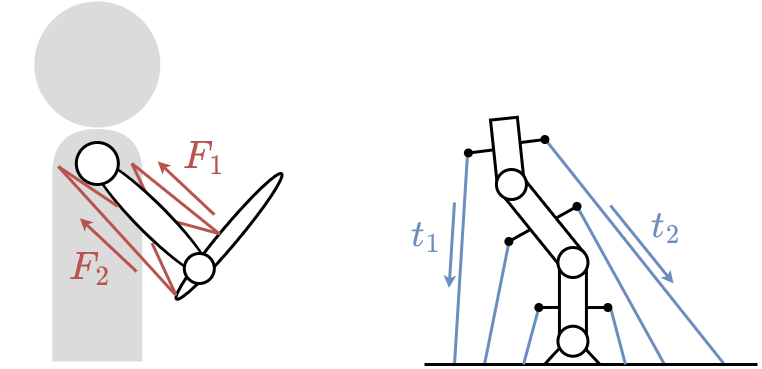
\includegraphics[width=0.45\linewidth]{Chapters/imgs/muscle_mcdrs.png}
    \caption{An illustrative planar example of a human musculoskeletal model and a Multi-link cable-driven robot (MCDR). On the left human arm is modeled with two joints and six muscles, where each muscle can apply contraction forces $F_i$. On the right, a MCDR robot is modeled with 3 joints and 6 cables, which can apply tension forces $t_i$.  }
    \label{fig:muscle_mcdrs}
\end{figure}

Multi-link cable-driven robots (MCDRs) \cite{Wang2019} are gaining momentum in recent years by combining the benefits of serial and parallel robots. They have relatively large workspace compared to parallel robots and much lower inertia than the serial robots, resulting in higher achievable velocities and better back-drivability. 

As this family of robots is actuated by cable actuators that are capable of applying unidirectional tensile forces, there is a natural parallel with musculoskeletal models. Lau et al. \cite{Lau2013} have even proposed a generalised modelling framework for MCDR modelling and demonstrated that it can be used for musculoskeletal models as well. An simplified planar example of a human musculoskeletal model and the MCDR model is shown on Figure \ref{fig:muscle_mcdrs}.

One of the main differences comes from the actuator point of view. When it comes to MCDRs, the dynamics of the actuators is often neglected, considering them capable of instantaneously applying a range of $d$ tensile forces $\bm{t}\in\mathbb{R}^d$.
\begin{equation}
    \bm{t} \in [\bm{0},~\bm{t}_{max}]
\end{equation}
Additionally, this range is often considered constant and is not state dependent. For musculoskeleral models, on the other hand, the ranges of achievable muscle tension forces $\bm{F}$ are subject to many different biomechanical and biological factors, such as muscle length $\bm{l}$ and extension velocity $\dot{\bm{l}}$ as well the effects of fatigue and temperature.
Therefore the cables of the MCDRs can be seen as idealised muscles which tensile force capacity stays constant. 

Consequently, the physical ability metrics defined for the musculoskeleral models have the same formulation as the ones used to asses the performance of MCDRs.

\subsubsection{Wrench/Force polytope}
\label{ch:force_poly_human}
Task space force (or more generally wrench) capacity $\bm{f} \in \mathbb{R}^m$ is a well established metrics in biomechanics. It has been defined in two manners, a simplified formulation where the torques of $n$ human joints $\bm{\tau} \in \mathbb{R}^n$ are considered independent and limited (\ref{eq:human_torque_lim}) and in a more complete form where the human's joint torques $\bm{\tau}$ are generated by $D$ muscle tensile forces $\bm{F} \in \mathbb{R}^d$ which are limited in their respective ranges (\ref{eq:muslce_initial_range}).

Torque based polytopes \cite{rezzoug_application_2012,sasaki2011vertex} of achievable task space wrenches $\bm{f}$ have the same formulation as the force polytopes for robotic manipulators described in Chapter \ref{ch:poly_force}. Therefore all the considerations for their evaluation are equivalent to those for robotic manipulators.  

However, real limits of human joint torques cannot be expressed as independent ranges (\ref{eq:human_torque_lim}) as they are generated by $d$ muscle tensile forces $\bm{F}$. The true limits of the joint torques $\bm{\tau}$ are polytope shaped as a consequence of the affine mapping of the muscle forces $\bm{F}$ to the joint space, though the moment arm matrix $N(\bm{q})=-L(\bm{q})^T$.
\begin{equation}
\mathcal{P}_\tau(\bm{q}) = \{\bm{\tau} \in \mathbb{R}^n ~|~\bm{F}\in [\bm{F}_{min}, \bm{F}_{max}], ~\bm{\tau}=N(\bm{q})\bm{F}\}
\label{eq:poly_torque_human}
\end{equation}

The relationship of the achievable task space wrenches $\bm{f}$ and the joint torques $\bm{\tau}$ is described through the dynamics equation 
\begin{equation}
\underbrace{M(\bm{q})\ddot{\bm{q}} + C(\bm{q},\dot{\bm{q}})\dot{\bm{q}} + \bm{g}(\bm{q})}_{\bm{\tau}_b(\bm{q},\dot{\bm{q}},\ddot{\bm{q}})} + J^T(\bm{q})\bm{f} = \bm{\tau} 
\end{equation}
where $\bm{\tau}_b(\bm{q},\dot{\bm{q}},\ddot{\bm{q}})$ is a state dependant joint torque bias vector including the influence of the gravity $\bm{g}(\bm{q})$ and human motion $\{\dot{\bm{q}},\ddot{\bm{q}}\}$. 

Finally the achievable set of task space wrenches $\bm{f}\in\mathbb{R}^m$ can then be expressed as a set of all the achievable wrenches $\bm{f}$ given the polytope $\mathcal{P}_\tau$ shaped limits of joint torques $\bm{\tau}$
\begin{equation}
    \mathcal{P}_f(\bm{q},\dot{\bm{q}},\ddot{\bm{q}}) = \left\{ \bm{f} \in \mathbb{R}^m ~|~ \bm{\tau}\in \mathcal{P}_\tau(\bm{q}), ~~ J^T(\bm{q})\bm{f} = \bm{\tau} -\bm{\tau}_b(\bm{q},\dot{\bm{q}},\ddot{\bm{q}}) \right\}
\end{equation}
Or in its implicit formulation
\begin{equation}
    \mathcal{P}_f(\bm{q},\dot{\bm{q}},\ddot{\bm{q}}) = \left\{ \bm{f} \in \mathbb{R}^m ~|~ \bm{F}\in\left[\bm{F}_{min}, \bm{F}_{max} \right], ~~ \!J^T(\bm{q})\bm{f} =\! N(\bm{q})\bm{F} -\bm{\tau}_b(\bm{q},\dot{\bm{q}},\ddot{\bm{q}}) \right\}
    \label{eq:human_force_poly}
\end{equation}

The final polytope formulation $\mathcal{P}_f$ has an implicit form composed of two affine mappings. First the limits of the muscle tension forces $\bm{F}\in \mathbb{R}^d$ are projected into the limits of the joint torques $\bm{\tau}\in \mathbb{R}^n$, then the polytope of the joint torques $\mathcal{P}_\tau$ is transformed to the task space wrenches $\bm{f}\in \mathbb{R}^m$ using the jacobian transpose matrix $J(\bm{q})^T$. As the musculoskeletal models often have large number of muscles $d$, the ending polytope $\mathcal{P}_f$ geometry is complex (having a large number of vertices and faces), both due to the number of muscles considered and the inherent complexity of the affine mapping. Therefore, this metric has been mostly used for static in-advance analysis of human postures \cite{hernandez_toward_2015}, due to its long execution times. 

However, Carmichael et al. \cite{carmichael_estimating_2013, carmichael2011Towards} have proposed a method capable of improving the time efficiency of the polytope resolution that has a potential to be used even in real-time applications. This method is based on Ray shooting method (RSM) that samples the polytope in a set of predefined direction in task space. By choosing the directions of interest in advance, the method is capable of approximating the polytope, however it does not give any guarantees on the approximation accuracy.

The achievable wrench polytope $\mathcal{P}_f$ formulation (\ref{eq:human_force_poly}) have been used for the analysis of the multi-link cable-driven robots (MCDRs) as well, for example in works by Sheng et al. \cite{sheng2020operational} or Muralidharan et al. \cite{Muralidharan2022}.

\subsubsection{Acceleration polytope}
\label{ch:human_aceleration_poly}

Task space acceleration polytope $\mathcal{P}_a$ describes the relationship between the limitation of the muscle tensile forces $\bm{F}\in \mathbb{R}^d$ and the set of achievable task space accelerations $\ddot{\bm{x}}\in\mathbb{R}^m$.

As in the case of the force polytope, the simplified approach to this metric is possible, where the human joint torque limits $\bm{\tau}\in\mathbb{R}^n$ are specified as independent ranges. Resulting in the formulation of the acceleration polytope identical to the one for robotic manipulators introduced in Chapter \ref{ch:accel_poly_robot}. 

However, human's joint torques $\bm{\tau}$ are not generated by a set of independent actuators, as in case of robotic systems, but with a set of $d$ contraction forces $\bm{F}$ produced by the muscle-tendon units $\bm{\tau}=N(\bm{q}) \bm{F}$. Therefore, real limits of achievable torques of human joints are polytope $\mathcal{P}_\tau$ shaped, as described by equation (\ref{eq:poly_torque_human}). 

The achievable acceleration polytope $\mathcal{P}_a$ formulation, respecting the muscle tension forces limits $\bm{F}$, can be derived from the human dynamics equation
\begin{equation}
M(\bm{q})\ddot{\bm{q}} + \underbrace{C(\bm{q},\dot{\bm{q}})\dot{\bm{q}} + \bm{g}(\bm{q}) + J^T(\bm{q})\bm{f}}_{\bm{\tau}_b(\bm{q},\dot{\bm{q}}, \bm{f})} = N(\bm{q}) \bm{F} 
\end{equation}
where $N(\bm{q})=-L(\bm{q})^T$ is the state dependant moment arm matrix. 
For any given human state $\{\bm{q},\dot{\bm{q}}, \bm{f}\}$, the effects of the human's motion, the gravity as well as the applied external wrenches, can be grouped in a constant torque vector $\bm{\tau}_b(\bm{q},\dot{\bm{q}},\bm{f})$. Then the actuator acceleration $\bm{q}$ can be expressed in relationship to the applied joint torque $\bm{\tau}$
\begin{equation}
    \ddot{\bm{q}} = M(\bm{q})^{-1}N(\bm{q})\bm{F} - M(\bm{q})^{-1}\bm{\tau}_b(\bm{q},\dot{\bm{q}}, \bm{f})
\end{equation}
Finally, the joint accelerations $\ddot{\bm{q}}$ can be transformed to the task space using the mapping (\ref{eq:js_to_cs_vaj_human:accel})
\begin{equation}
    \ddot{\bm{x}} = J(\bm{q})M(\bm{q})^{-1}N(\bm{q})\bm{F} - \underbrace{J(\bm{q})M(\bm{q})^{-1}\bm{\tau}_b(\bm{q},\dot{\bm{q}},\bm{f}) + \dot{J}(\bm{q}, \dot{\bm{q}})\dot{\bm{q}}}_{\bm{a}_b(\bm{q},\dot{\bm{q}},\bm{f})}
\end{equation}
where $\bm{a}_b(\bm{q},\dot{\bm{q}},\bm{f}) \in \mathbb{R}^m$ presents a constant bias vector for any human joint state $\{\bm{q},\dot{\bm{q}},\bm{f}\}$. The polytope $\mathcal{P}_a$ of achievable task space accelerations $\ddot{\bm{x}}$ can then be expressed as
\begin{equation}
\begin{split}
    \mathcal{P}_a(\bm{q},\dot{\bm{q}},\bm{f}) = \{ \ddot{\bm{x}} \in \mathbb{R}^m ~|~ \bm{F}&\in\left[\bm{F}_{min}, \bm{F}_{max} \right],\\ \ddot{\bm{x}} &= J(\bm{q})M(\bm{q})^{-1}N(\bm{q})\bm{F} - \bm{a}_b(\bm{q},\dot{\bm{q}},\bm{f}) \}
\end{split}
\end{equation}
The polytope $\mathcal{P}_a$ is formulated as a linear and affine projection of the muscles tension force $\bm{F}$ limits using the state dependant projection matrix $J(\bm{q})M(\bm{q})^{-1}N(\bm{q})$.  This polytope is much simpler to resolve than the force polytope $\mathcal{P}_f$ as it represents a projection of the $d$ dimensional limits of mucsle tension forces $\bm{F}$ to the lower $m$ dimensional space of achievable task space accelerations $\ddot{\bm{x}}$.

Polytope $\mathcal{P}_a$ metrics have been used for musculoskeletal model analysis of highly dynamical movements such as football throwing \cite{khatib2009robotics} and golf swinging \cite{demircan2012muscle}. Additionally this metric has been used for the design analysis of the multi-link cable driven robots (MCDRs) as well \cite{sheng2020operational}.

\subsubsection{Velocity polytope}

The simplest form of task space velocity capacity describes the relationship between the limited ranges (\ref{eq:human_js_vel_lim}) of human joint velocity $\dot{\bm{q}} \in \mathbb{R}^n$ and achievable task space velocities $\dot{\bm{x}} \in \mathbb{R}^m$, mapped through the jacobian matrix $J(\bm{q}) \in \mathbb{R}^{m\times n}$.
\begin{equation}
    \mathcal{P}_v(\bm{q}) = \left\{ \dot{\bm{x}} \in \mathbb{R}^m ~|~ \dot{\bm{q}}\in\left[\dot{\bm{q}}_{min}, \dot{\bm{q}}_{max} \right], ~~ \dot{\bm{x}} = J(\bm{q})\dot{\bm{q}} \right\}
\end{equation}
This formulation is essentially the same as the one for robotic manipulators described in Chapter \ref{ch:vel_poly} and all the considerations discussed in that chapter are valid for this formulation as well.

However, taking in account only human's joint velocity $\dot{\bm{q}}$ limits in a form of independent ranges (\ref{eq:human_js_vel_lim}) does not take in consideration the limits of muscle extension velocity $\dot{\bm{l}}\in\mathbb{R}^d$. The true limits of human joint velocities are configuration dependent, as they are a consequence of the limits of muscle extension velocities $\dot{\bm{l}}$. The relationship between the joint and muscle extension velocities is given through the muscle jacobian matrix $L(\bm{q}) \in \mathbb{R}^{d\times n}$, forming polytope shaped limits
\begin{equation}
    \mathcal{P}_{\dot{q}}(\bm{q}) = \left\{ \dot{\bm{q}} \in \mathbb{R}^n ~|~ \dot{\bm{l}}\in\big[\dot{\bm{l}}_{min}, \dot{\bm{l}}_{max} \big], ~~ L(\bm{q})\dot{\bm{q}} = \dot{\bm{l}} \right\}
    \label{eq:human_poly_joint_vel}
\end{equation}
These polytope shaped limits can then be used to define the achievable task space velocity $\dot{\bm{x}}\in \mathbb{R}^m$ polytope which respects the limits of the muscle extension velocity $\dot{\bm{l}}$.
\begin{equation}
    \mathcal{P}_v(\bm{q}) = \left\{ \dot{\bm{x}} \in \mathbb{R}^m ~|~ \dot{\bm{q}}\in  \mathcal{P}_{\dot{q}}(\bm{q}), ~~ J(\bm{q})\dot{\bm{q}} = \dot{\bm{x}} \right\}
\end{equation}
Or in its implicit form
\begin{equation}
    \mathcal{P}_v(\bm{q}) = \left\{ \dot{\bm{x}} \in \mathbb{R}^m ~|~ \dot{\bm{l}}\in\big[\dot{\bm{l}}_{min}, \dot{\bm{l}}_{max} \big], ~~ J(\bm{q})\dot{\bm{q}} = \dot{\bm{x}}, ~~ L(\bm{q})\dot{\bm{q}} = \dot{\bm{l}} \right\}
    \label{eq:velocity_polytope_human}
\end{equation}

This metric has an implicit formulation making its resolution relatively complex, requiring using multiple standard methods for polytope evaluation. It first requires finding the limits of joint velocities $\dot{\bm{q}} \in \mathbb{R}^n$ based on the limits of the muscle extension velocities $\dot{\bm{l}} \in \mathbb{R}^d$ and then projecting them to the task space velocities $\dot{\bm{x}} \in \mathbb{R}^m$. 

To the best of our knowledge, polytope $\mathcal{P}_v$ in its full implicit form (\ref{eq:velocity_polytope_human}), has not yet been used with musculoskeletal models. However, achievable velocity based physical ability metrics such as manipulability ellipsoids considering the joint velocity $\dot{\bm{q}}$ limits \cite{Chiu1988,Petric2019,Yang2017}, have been used in the human motion and ergonomics analysis. However, as these metrics neglect the the muscle extension velocity $\dot{\bm{l}}$ limits, polytope $\mathcal{P}_v$ could be used as their more complete alternative. 

The achievable velocity polytope $\mathcal{P}_v$, in the form (\ref{eq:velocity_polytope_human}), has been used for multi-link cable driven robots (MCDRs) analysis \cite{Muralidharan2022}.

\subsubsection{Stiffness polytope}
\label{ch:human_stiffness_poly}
Stiffness metrics for human musculoskeletal models are used to evaluate the limitations of the endpoint displacement $\Delta x \in \mathbb{R}^m$ given the known muscle stiffness matrix $K_m \in \mathbb{R}^{d\times d}$ and a limited range of task space wrenches $\bm{f} \in \mathbb{R}^m$. 

\begin{equation}
    \bm{f}\in\left[\bm{f}_{min}, \bm{f}_{max} \right]
    \label{eq:force_stiff_range_human}
\end{equation}

With a known muscle stiffness matrix $K_m$, that can be determined using the Hill's muscle model \cite{LATASH1993653}, the joint stiffness matrix $K_j\in \mathbb{R}^{n\times n}$ can be found using the muscle jacobian matrix $L(\bm{q}) \in \mathbb{R}^{d\times n}$
\begin{equation}
    K_j = L(\bm{q}) K_m L(\bm{q})^T 
\end{equation}
This joint space stiffness matrix $K_j$ can be used to find the robot state dependent task space stiffness $K_c  \in \mathbb{R}^{m\times m}$, through the jacobian matrix $J(\bm{q})\in\mathbb{R}^{m\times n}$  \cite{Salisbury1980,Ajoudani2018,Inouye2016}
\begin{equation}
     K_c(\bm{q}) = (J(\bm{q}) K_j^{-1}J(\bm{q})^T)^{-1}
\end{equation}
Given the range of expected external wrenches (\ref{eq:force_stiff_range_human}), the polytope of maximal achievable displacements $\Delta\bm{x}$ can then be expressed as
\begin{equation}
    \mathcal{P}_\Delta(\bm{q}) = \left\{ \Delta\bm{x} \in \mathbb{R}^m ~|~ \bm{f}\in\left[\bm{f}_{min}, \bm{f}_{max} \right], ~~ \Delta\bm{x} = K_c(\bm{q})^{-1}\bm{f} \right\}
    \label{eq:stiffness_human_simple}
\end{equation}


However, this formulation considers that the external wrench $\bm{f}$ range (\ref{eq:force_stiff_range_human}) is inside the human wrench capacity. In order to make sure that the human's wrench capacity is not exceeded when calculating the maximal achievable displacement polytope $\mathcal{P}_\Delta$ the external wrench range (\ref{eq:force_stiff_range_human}) needs to be intersected with the human's wrench polytope  $\mathcal{P}_f$ described in the Chapter \ref{ch:force_poly_human}, the polytope $\mathcal{P}_\Delta$ of achievable task space displacement $\Delta \bm{x}$ can then be expressed as
\begin{equation}
    \mathcal{P}_\Delta(\bm{q},\dot{\bm{q}},\ddot{\bm{q}}) = \left\{ \Delta\bm{x} \in \mathbb{R}^m ~|~ \bm{f}\in \left[\bm{f}_{min}, \bm{f}_{max} \right] \cap \mathcal{P}_f(\bm{q},\dot{\bm{q}},\ddot{\bm{q}}),  ~~ \! \Delta\bm{x}=K_c(\bm{q})^{-1}\bm{f}\right\}
\end{equation}

If the maximal displacement polytope $\mathcal{P}_\Delta$ is calculated only in relationship to the human's wrench capacity $\mathcal{P}_f$, without specifying the expected range of external wrenches (\ref{eq:force_stiff_range_human}), this polytope can be expressed in an implicit form
\begin{equation}
\begin{split}
    \mathcal{P}_\Delta(\bm{q},\dot{\bm{q}},\ddot{\bm{q}}) =\! \{ \Delta\bm{x} \in \mathbb{R}^m ~|&\bm{F}\in\left[\bm{F}_{min}, \bm{F}_{max} \right]\!,\\ ~ &J^T(\bm{q})K_c(\bm{q})\Delta\bm{x}\!= N(\bm{q})\bm{F}\! -\! \bm{\tau}_b(\bm{q},\dot{\bm{q}},\ddot{\bm{q}}) \}\label{eq:stiffness_human_all}
\end{split}
\end{equation}
The stiffness polytope $\mathcal{P}_\Delta$ then represents the maximal task space displacement $\Delta \bm{x} \in \mathbb{R}^m$ that can be achieved given the human's muscle tensile forces $\bm{F} \in \mathbb{R}^d$ limits (\ref{eq:muslce_initial_range}), this polytope formulation is also called \textit{stiffness feasibility region} \cite{ajoudani2017choosing}.

The formulation of the polytope (\ref{eq:stiffness_human_simple}) has relatively low complexity, defined as a projection of the limits of the external task space wrenches $\bm{f} \in \mathbb{R}^m$ to the same dimensional task space displacements $\Delta \bm{x} \in \mathbb{R}^m$. However, the implicit polytope formulation (\ref{eq:stiffness_human_all}) is much more complex as the limits of muscle tension forces $\bm{F} \in \mathbb{R}^d$ first need to be projected to the limits of the joint torques $\bm{\tau} \in \mathbb{R}^n$ which in term determine the set of achievable displacements $\Delta \bm{x} \in \mathbb{R}^m$. While the formulation  (\ref{eq:stiffness_human_simple}) can be resolved with standard polytope resolution algorithms, the formulation (\ref{eq:stiffness_human_all}) requires a combination of multiple methods, making it significantly more time consuming. 

These polytope based metrics however, to the best of our knowledge, have yet to be used with human musculoskeletal models and MCDRs. However, their potential has already been shown for human posture analysis \cite{Inouye2016} and MCDR design \cite{Ramadoss2021} applications, in their simplified ellipsoid forms.

\subsection{Collaboration metrics}
\label{ch:collab_metrics}

\begin{figure}[!h]
    \centering
    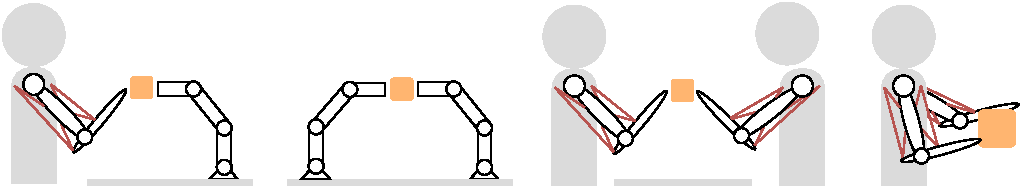
\includegraphics[width=\linewidth]{Chapters/imgs/collaboration.pdf}
    \caption{Illustrative examples of different collaboration scenarios, from left to right, human-robot, robot-robot, human-human and even two arms of a human subject can be seen as a collaboration of two musculoskeletal models.}
    \label{fig:collaboration_types}
\end{figure}

Physical ability metrics are an important tool for analysing how robots and humans comply with different requirements of tasks. In human-robot collaboration scenarios, these metrics can be used is to decide if the robot, or the human, is better suited to execute a certain task, by evaluating their different physical abilities (movement, forces, precision etc.) to the ones required by the task. 

However, when it comes to the physical collaboration, where the task is executed jointly by the human and the robot physically interacting, expressing their common phisical abilities is much more challenging. As their common physical ability is a combination of their individual abilities, to be able to calculate their common physical ability, they need to be expressed in a unified form.

Expressing the physical ability metrics, for both humans and robots, in the polytope form, enables using the polytope algebra to do different operations, such as sum, intersection and union, which are well defined and can be calculated efficiently. Combining the individual polytopes using the polytope algebra can be used to describe different physical collaboration scenarios and enables characterisation of the common physical abilities of the collaboration in the convex polytope form as well.

One example of such metric has been developed by Jihong Lee, in his work \cite{lee2001velocity}, showing how polytopes can be used to describe the common velocity capacity of multi-arm collaborative robotic system.

Following two chapters, \ref{ch:force_collab} and \ref{ch:velocity_collab}, describe the calculation of common force and velocity capacity of a physical human-robot collaboration based on polytope algebra. Similar polytope operations can be used to calculate other polytope based physical ability metrics, such as precision, stiffness or acceleration. Furthermore, similar approach can be used to characterise different collaboration scenarios. Finally, these metrics are not specific to human-robot collaboration, and can be used for scenarios with multiple robots and multiple humans as well. Even the interaction of the two arms of the human subject can be seen as an collaboration scenario and the same approaches can be used to determine their common physical abilities. Simplified visual examples of different collaboration scenarios are shown on Figure \ref{fig:collaboration_types}.

\subsubsection{Force polytope}
\label{ch:force_collab}
\begin{figure}[!h]
    \centering
    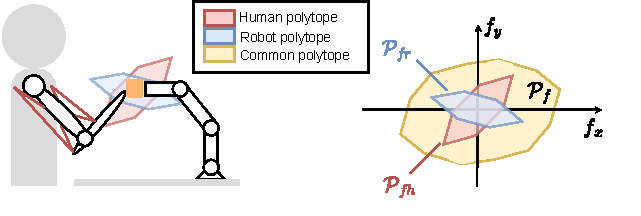
\includegraphics[width=0.7\linewidth]{Chapters/imgs/force_collab.pdf}
    \caption{A collaborative example scenario where a human and a robot interact over an object fixed rigidly in the end-effector of the robot and in the hand of the human. The force polytope of the human (red) and the robot (blue) as well as their collaborative polytope (orange) calculated as a minkowski sum of their individual polytopes are shown on the right.}
    \label{fig:collaboration_force}
\end{figure}

If for example, a human operator and a robot are physically interacting in order to manipulate an object which is rigidly fixed both in the robot's end-effector and the human hand, the final force exerted on the object will be the sum of the forces of the human $\bm{f}_h$ and the force of the robot $\bm{f}_r$.
\begin{equation}
    \bm{f} = \bm{f}_h + \bm{f}_r
\end{equation}

Their individual force capacity can be expressed in a polytope form, for the human  $\mathcal{P}_{fh}$ and the robot  $\mathcal{P}_{fr}$ respectively. Finally, as their forces acting on the object are summed, their common force capacity on the object can be calculated as the Minkowski sum of the polytopes
\begin{equation}
    \mathcal{P}_f =  \mathcal{P}_{fh} \oplus \mathcal{P}_{fr}
\end{equation}
A planner example of this collaboration scenario and the polytopes obtained is in shown on Figure \ref{ch:force_collab}. 

In more general case, if a collaboration is composed of $N$ actors rigidly holding an object, where their force capacity is expressed in a polytope form $\mathcal{P}_{fi}$, then their common force capacity can be calculated as the Minkowski sum of the $N$ polytopes.

\begin{equation}
    \mathcal{P}_f =  \mathcal{P}_{f1} \oplus \mathcal{P}_{f2} \oplus ~\ldots ~\oplus  \mathcal{P}_{fN}
\end{equation}

\subsubsection{Velocity polytope}
\label{ch:velocity_collab}
\begin{figure}[!h]
    \centering
    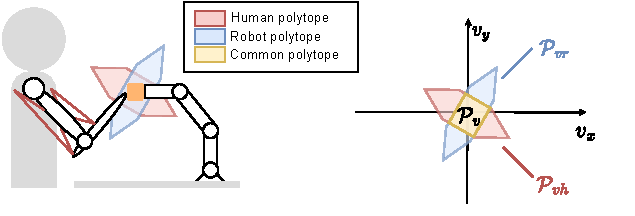
\includegraphics[width=0.7\linewidth]{Chapters/imgs/velocity_collab.pdf}
    \caption{A collaborative example scenario where a human and a robot interact over an object fixed rigidly in the end-effector of the robot and in the hand of the human. The velocity polytope of the human (red) and the robot (blue) as well as their collaborative polytope (orange) calculated as an intersection of their individual polytopes are shown on the right.}
    \label{fig:collaboration_vel}
\end{figure}

If the same example as for the force capacity \ref{ch:force_collab} is considered, where a human operator and a robot are physically interacting in order to manipulate an object which is rigidly fixed both in the robot's end effector and the human hand. The maximal velocity the object can achieve in a certain direction $\bm{v}_{max}$ will be limited by the actor who has the lower maximal velocity in that direction. It can be found as the minimum value of the maximal velocity the human arm can achieve $\bm{v}_{h,max}$ and the robot's end-effector can achieve $\bm{v}_{r,max}$
\begin{equation}
    \bm{v}_{max}= \min \{\bm{v}_{h,max}, \bm{v}_{r,max}\}
\end{equation}

Once their individual velocity capacity is expressed in polytope form $\mathcal{P}_{vh}$ and $\mathcal{P}_{vr}$, their common velocity capacity $\mathcal{P}_v$ (the achievable velocities of the object) can then be calculated as the intersection of their polytopes
\begin{equation}
    \mathcal{P}_v =  \mathcal{P}_{vr} \cap \mathcal{P}_{vh}
\end{equation}

In a more general case where there are $N$ actors (robots and humans) collaborating by rigidly holding the object, and where their velocity capacity is expressed in a polytope form $\mathcal{P}_{vi}$, the common velocity capacity can be calculated as their intersection
\begin{equation}
    \mathcal{P}_v =  \mathcal{P}_{v1} \cap \mathcal{P}_{v2} \cap ~~ \ldots ~~\cap \mathcal{P}_{vN}
\end{equation}

A planner example of this collaboration scenario and the polytopes obtained is in shown on Figure \ref{ch:velocity_collab}. 


\section{Generic view on common polytope formulations}
\label{ch:generic_view}

Physical ability metrics describe the relationship between the different actuator limits (joint torques $\bm{\tau} \in \mathbb{R}^n$, joint velocities $\dot{\bm{q}} \in \mathbb{R}^n$, muscle forces $\bm{F} \in \mathbb{R}^d$, extension velocities $\dot{\bm{x}} \in \mathbb{R}^d$, etc.) and achievable sets of different task related variables (velocities $\dot{\bm{x}}$, accelerations $\ddot{\bm{x}}$, wrenches $\bm{f}$, etc.). In order to obtain the polytope shaped achievable sets, in general case, both robots' and humans' (based on musculoskeletal models) dynamics and kinematics equations are be linearised around a certain state $\{\bm{q},\dot{\bm{q}},\ddot{\bm{q}} \}$, producing linear and affine transformations of the actuator limits to the desired cartesian variables. 

Physical ability polytopes can then be seen as the set of feasible output variables $\bm{x} \in \mathbb{R}^m$ produced by applying an affine transformation of the input variables $\bm{y} \in \mathbb{R}^n$, bounded within the convex input set $\bm{y}\in\mathcal{I}$. The input space $\mathcal{I}$ in the case of physical ability metrics is usually higher-dimensional the the output space $n\geq m$ and often defined as a hypercube (min-max intervals) 
\begin{equation}
    \mathcal{I} = \{\bm{y} |~~ \bm{y}_{min} \leq \bm{y}\leq \bm{y}_{max} \}
    \label{eq:hypercube_lim}
\end{equation}
or in more general case a convex polytope (set of linear constraints).
\begin{equation}
    \mathcal{I} = \{\bm{y} |~~ H\bm{y}\leq \bm{d} \}
\end{equation}


The physical ability metrics are then defined as affine transformations of the set $\mathcal{I}$, resulting in a convex polytope $\mathcal{P}_x$. There are two main families of polytope types based on their affine mapping formulation 

\begin{itemize}
    \item Projection formulation: 
    \begin{equation}
        \mathcal{P}_x=\{\bm{x} |~ \bm{x} = B\bm{y} + \bm{c},~\bm{y} \in\mathcal{I} \}
        \label{eq:proj_poly}
    \end{equation}
    \item Intersection formulation: 
    \begin{equation}
        \mathcal{P}_x=\{\bm{x} |~ A\bm{x} = \bm{y}+ \bm{c},~ \bm{y} \in \mathcal{I}\}
        \label{eq:inter_poly}
    \end{equation}
\end{itemize}
Where $A\in \mathbb{R}^{n\times m }$ and $B\in \mathbb{R}^{m\times n}$ are matrices mapping the $n$ dimensional input space and $m$ dimensional output space  and $\bm{c} \in \mathbb{R}^n$ is a constant bias vector.

\subsection{Projection and intersection formulation}
The distinction between the intersection and projection formulation is important only if the matrices $A\in \mathbb{R}^{n\times m }$ and $B\in \mathbb{R}^{m\times n}$ do not have a full rank ($n\!>\!m$). If the matrices have full rank ($n\!=\!m$), the intersection formulation $A\bm{x} = \bm{y} + \bm{c}$ can be transformed to the projection formulation $\bm{x} = A^{-1}(\bm{y}+\bm{c})$, as the matrix $A$ is square  and invertible.  

In the case where the matrix $A$ does not have a full rank ($n\!>\!m$), as the matrix $A$ is no longer invertible, this manipulation is no longer possible, requiring different approach for its resolution. As the physical ability metrics in most cases map the higher dimensional space (ex. joint space or muscle force space) to the lower dimensional output space (ex. 3D Cartesian space), the condition $n\!>\!m$ corresponds to the common case where the redundant degrees of freedom are present. 


\begin{figure}
    \centering
    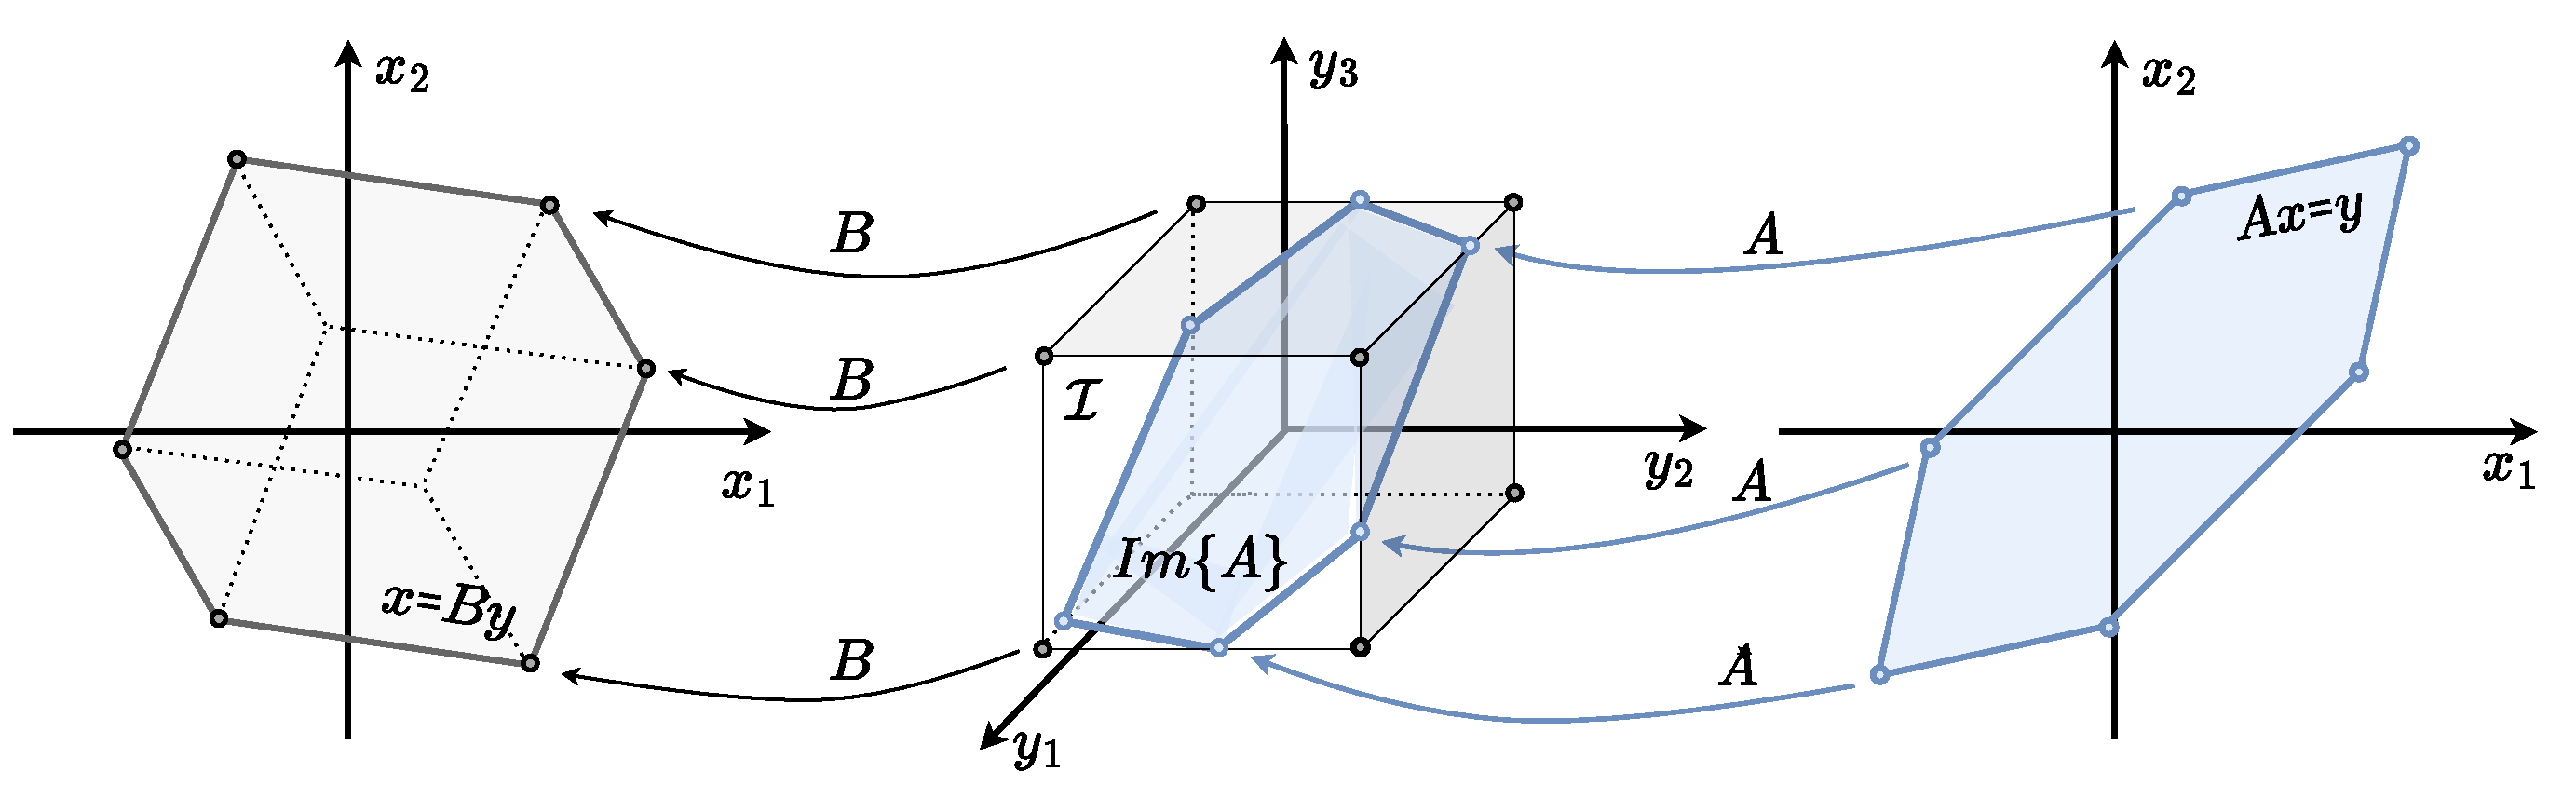
\includegraphics[width=\linewidth]{Chapters/imgs/intersection_projection.pdf}
    \caption{A comparative view of the projection (left) and intersection (right) polytope formulation using the same input space (middle). In the projection formulation, the whole input space $\mathcal{I}$ is projected using the matrix $B$ to the output space to obtain the polytope $\mathcal{P}_x$ (gray left). In the intersection formulation, first the intersection of the input space $\mathcal{I}$ with the image of the matrix $A$ has to be found (blue middle) $Im\{A\} \cap \mathcal{I}$ , then this intersection can be projected to the output space using the inverse of the matrix $A$ to obrain the polytope $\mathcal{P}_x$ (blue right).}
    \label{fig:inter_proj}
\end{figure}

Figure \ref{fig:inter_proj} shows the difference between the formulation types on an example of a $n=3$ dimensional input space and $m=2$ dimensional output space, where the bias $\bm{c}$ is a zero vector $\bm{0}$.
Projection formulation polytope is an affine transformation (projection $\bm{x}=B\bm{y}$) of the $n$-dimensional input space $\mathcal{I}$ to the $m$-dimensional output space. As the projection is linear the vertices and the faces of the of the polytope $\mathcal{P}_x$ are a subset of projected vertices and faces of the space $\mathcal{I}$. The intersection formulation polytope is defined as an affine transformation (projection $\bm{y}=A\bm{x}$) of the  lower dimensional output space to the higher dimensional input space, therefore an inverse of the projection formulation.

\paragraph*{From intersection to projection formulation} The main difficulty of the intersection formulation (\ref{eq:inter_poly}) is that it is defined as an inverse projection, from the low dimensional output space to the high dimensional input space, as shown graphically on Figure \ref{fig:inter_proj}. 

Therefore, the achievable set of the output variables $\bm{x}\in \mathcal{P}_x$, defined as in the intersection formulation (\ref{eq:inter_poly}), will be entirely generated by the input variables $\bm{y}\in \mathbb{R}^n$, that can be described by the mapping $\bm{y} = A \bm{x}$. This relationship $\bm{y} = A \bm{x}$ defines an $m$ dimensional subspace of the $n$ dimensional input space, which is also called the image of the matrix $A$. 
\begin{equation}
    \bm{y}=A\bm{x} \in Im \{A\}
\end{equation}
The set of all the input variables $\bm{y}$ belonging to the projection $\bm{y} = A \bm{x}$ and the limitations $\bm{y}\in\mathcal{I}$ can then be found as their intersection
\begin{equation}
   \bm{y} \in Im\{A\} \cap \mathcal{I}
    \label{eq:intersection_ai}
\end{equation}

Once the new input space defined by the intersection (\ref{eq:intersection_ai}) is found, the achievable output space polytope $ \bm{x}\in\mathcal{P}_x$ can be found by the inverse projection $\bm{x}=A^{-1}\bm{y}$. As in general case, the matrix $A$ is not invertible ($n>m$), the Moore-Penrose pseudo-inverse of the matrix $A^+ = A^T(AA^T)^{-1}$ can be used. The pseudo-inverse $A^+$ can be used as the unique inverse projector from the input to the output space because for all the input variables $\bm{y}$ described by the equation (\ref{eq:intersection_ai}) as they all belong to the image of the matrix $A$. 
\begin{equation}
    \bm{x} = A^+ \bm{y}, \quad \bm{y} \in Im\{A\}\cap\mathcal{I}
\end{equation}

Therefore,  by exploiting this relationship,  the equivalent projection formulation of the the initial intersection polytope formulation (\ref{eq:inter_poly}) can be expressed
\begin{equation}
\mathcal{P}_x=\{\bm{x} |~ \bm{x} = A^+\bm{y},~ \bm{y} \in Im\{A\}\cap\mathcal{I}\} \label{eq:proj_inter}
\end{equation}
Figure \ref{fig:inter_proj} shows a graphical representation of this mapping where the intersection (\ref{eq:intersection_ai}) is shown in blue, as well as the final polytope $\mathcal{P}_x$ being its projection to the output space $\bm{x}\in \mathbb{R}^m$. 

If the bias vector $\bm{c}$ is not a zero vector the complete formulation becomes
\begin{equation}
\mathcal{P}_x=\{\bm{x} |~ \bm{x} = A^+\bm{y} - A^+\bm{c},~ \bm{y} - \bm{c}\in Im\{A\}\cap\mathcal{I}\} 
\end{equation}

Therefore, the intersection formulation (\ref{eq:inter_poly}) is generally more computationally complex to work with than the projection formulation, as it requires characterising the intersection $Im\{A\}\cap\mathcal{I}$. 

% \subsection{Combined formulation}

% A special case of intersection formulation (\ref{eq:inter_poly}), that occurs when calculating wrench capacity and stiffness capacity of human musculoskeletal models, arises when the input space has a projection formulation (\ref{eq:proj_poly}). 
% The resulting polytope has a combined intersection and projection formulation
% \begin{equation}
%     \mathcal{P}_x \in \{\bm{x}~|~A \bm{x} = B \bm{y} + \bm{c},~ \bm{y} \in \mathcal{I}\} 
% \end{equation}
% where $\bm{x}\in\mathbb{R}^m$ is the output vector, $\bm{y} \in \mathbb{R}^d$ is an input vector, matrix $B\in \mathbb{R}^{n \times d}$ is a projector matrix from $d$ dimensional input space to the $n$ dimensional intermediate space, matrix $A\in \mathbb{R}^{n\times m}$ is a projector matrix from $m$ dimensional output space to the $n$ dimensional intermediate space and $\bm{c}\in\mathbb{R}^n$ is the bias vector.

% The combined formulation can be transformed to the projection formulation as well using the same procedure as for the intersection formulation, resulting in a formulation
% \begin{equation}
% \mathcal{P}_x=\{\bm{x} |~ \bm{x} = A^+B\bm{y} - A^+\bm{c},~ B\bm{y} - \bm{c}\in Im\{A\}\cap\mathcal{I}\} 
% \end{equation}
% This polytope formulation is much more computationally complex than both intersection and projection formulation, as it requires first computing the projection $B\bm{y}$ and then the intersection $B\bm{y} \in Im\{A\}\cap\mathcal{I}$. 

\subsection{Categorising the polytope based metrics}
\label{ch:which_metric_which}

This chapter brings a classification of the common polytope based physical ability metrics for robotic systems, described in chapter \ref{ch:robot_metrics}, and for humans, described in chapter \ref{ch:human_metrics}, into four groups with respect to their formulation and input space shape.

All the described polytope metrics can be classified within two formulations: intersection and projection formulation. 
Examples of the intersection formulation for robotic systems are wrench polytope \ref{ch:poly_force} and stiffness region polytope \ref{ch:robot_stiffness_poly}, where the matrix $A$ corresponds to the jacobian transpose matrix $J(\bm{q})^T$. For the human musculoskeletal models the same metrics, wrench polytope \ref{ch:force_poly_human} and stiffness region polytope \ref{ch:human_stiffness_poly}, are examples of intersection formulation, and again the matrix $A$ corresponds to their jacobian transpose matrices $J(\bm{q})^T$. All the other metrics, both for humans and robots belong to the projection formulation.

With respect to the input space limits $\mathcal{I}$, there are two classes of metrics: ones with hypercube limits (min-max ranges) and the others with polytope limits. All the robot metrics introduced in chapter \ref{ch:robot_metrics} have hypercube limits, while in the case of human musculoskeletal models the only one with hypercube limits is the acceleration polytope \ref{ch:human_aceleration_poly}. Wrench, velocity and stiffens region polytope based on musculoskeletal models have polytope shaped input space $\mathcal{I}$. Wrench and stiffness region polytope have input space $\bm{y}$ corresponding to the space of joint joint torques $\bm{\tau}$, which belonging to the polytope of achievable joint torques $\mathcal{P}_\tau$ (\ref{eq:poly_torque_human}). The velocity polytope has input space $\bm{y}$ corresponding to the space of joint velocities $\dot{\bm{q}}$ belonging to the joint velocity polytope $\mathcal{P}_{\dot{\bm{q}}}$ (\ref{eq:human_poly_joint_vel}).


\begin{figure}[!h]
    \centering
    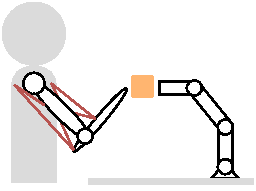
\includegraphics{Chapters/imgs/example_inter.pdf}
    \caption{A collaborative example scenario where a human and a robot interact over an object fixed rigidly in the end-effector of the robot and in the hand of the human.}
    \label{fig:table_inter}
\end{figure}

The polytope metrics can also be classified with respect to the polytope algebra operation necessary to combine multiple polytopes in order to calculate joint physical abilities. The collaboration scenario chosen for this comparison, is the same as in chapter \ref{ch:collab_metrics}, where a human operator and a robot are physically interacting in order to manipulate an object which is rigidly fixed both in the robot's end-effector. The example scenario is shown on Figure \ref{fig:table_inter}.

 
\begin{table}[!b]
\centering
\begin{tabular}{|l|c | c| c| c|}
\hline
Polytope Metric & Formulation & Input type & Dynamics & Collaboration \\
\hline
 \multicolumn{5}{c}{Robotic manipulators }  \\
\hline
Force/Wrench  & $Ax=y $ & $y\in \ [y_{min}, y_{max}]$ & Yes &$\oplus$ \\
Velocity  & $x=By$ & $y\in \ [y_{min}, y_{max}]$ & No & $\cap$ \\
Precision  & $x=By$ & $y\in \ [y_{min}, y_{max}]$ & No&  $\cap$ \\
Acceleration  & $x=By$ & $y\in \ [y_{min}, y_{max}]$& Yes &   $\cap$ \\
Jerk  & $x=By$ & $y\in \ [y_{min}, y_{max}]$& No &  $\cap$ \\
Stiffness feasibility  & $Ax=y$ & $y\in \ [y_{min}, y_{max}]$ & Yes& $\oplus$ \\
\hline
 \multicolumn{5}{c}{Human musculoskeletal models}  \\
\hline
Force/Wrench & $Ax=y$ & $y\in \mathcal{P}_y$ & Yes & $\oplus$ \\
Acceleration  & $x=By$ & $y\in \ [y_{min}, y_{max}]$& Yes &  $\cap$ \\
Velocity  & $x=By$ & $y\in \mathcal{P}_y$ & No &  $\cap$ \\
Stiffness feasibility  & $Ax=y$ & $y\in \mathcal{P}_y$  & Yes&  $\oplus$ \\
\hline
\end{tabular}
\caption{Comparison of polytope based physical ability metrics based on their formulation, input type, dynamics or kinematics formulation and their polytope algebra operator for a simple collaborative scenario on Figure \ref{fig:table_inter}.}
\label{tab:table_comparisson}
\end{table}


The physical ability metrics that require calculating wrench/force capacity polytope are going to be combined using minkowski sum operation $\oplus$. As in the example collaboration scenario, the cumulative wrenches applied on the object are a sum of human's and robot's applied wrenches, their common physical abilities are summed too. Such metrics are human's and robot's wrench polytope and stiffness region polytope. 
On the other hand, the physical ability metrics that are based on evaluating different robot's  and human's motion capacity will be combined using intersection operation $\cap$, as the common movement capacity of the collaboration will always be limited by the slowest actor (human or the robot). These metrics include velocity, precision, acceleration and jerk polytope for robots and acceleration and velocity polytopes for humans.

The classification of the described polytope based metrics, with respect to different formulation, input type, kinematic or dynamics conditions and collaboration operator, is shown in Table \ref{tab:table_comparisson}.

% \begin{table}
% \centering
% \begin{tabular}{|l|c|c|c|c|c| c| c|}
% \hline
% Polytope Metric & x & A & B & y & c & Dynamics & Collaboration \\
% \hline
%  \multicolumn{5}{c}{Robotic manipulators }  \\
% \hline
% Force/Wrench  & $\bm{f}$ & $J^T$ & - & $\bm{\tau}$ & $\bm{\tau}_b$ & Yes &$\oplus$ \\
% Velocity  & $\dot{\bm{x}}$ & - & $J$ & $\dot{\bm{q}}$ & - & No & $\cap$ \\
% Precision  & $\delta\dot{\bm{x}}$ & - & $J$ & $\delta\dot{\bm{q}}$ & - & No&  $\cap$ \\
% Acceleration  & $\ddot{\bm{x}}$ & - & $JM^{-1}$ & $\dot{\bm{\tau}}$ & $\bm{\tau}_b$ & Yes &   $\cap$ \\
% Jerk   & $\dddot{\bm{x}}$ & - & $J$ & $\dddot{\bm{q}}$ & $\bm{j}_b$ & No & $\cap$ \\
% Stiffness feasibility  & $\Delta\bm{x}$ & $J^T$ & - & $\bm{\tau}$ & $\bm{\tau}_b$ & Yes &$\oplus$ \\
% \hline
%  \multicolumn{5}{c}{Human musculoskeltal models}  \\
% \hline
% Force/Wrench & $\bm{f}$ & $J^T$ & $N$ & $\bm{F}$ & $\bm{\tau}_b$ & Yes &$\oplus$ \\
% Acceleration  & $\ddot{\bm{x}}$ & - & $JM^{-1}N$ & $\dot{\bm{\tau}}$ & $\bm{\tau}_b$ & Yes &   $\cap$ \\
% Velocity  & $\dot{\bm{x}}$ & - & $J$ & $\dot{\bm{q}}$ & - & Yes &   $\cap$ \\
% Stiffness feasibility  &$\Delta\bm{x}$ & $J^T$ & $N$ & $\bm{F}$ & $\bm{\tau}_b$ & Yes &$\oplus$ \\
% \hline
% \end{tabular}
% \caption{Polytope bases physical ability metrics comparison}
% \label{tab:my_label}
% \end{table}

% \begin{table}
% \centering
% \begin{tabular}{|l|c | c| c| c|}
% \hline
% Metric & Problem type & Input type & Dynamics & \begin{minipage}{3cm} \centering Collaboration \\ Serial/Parallel\end{minipage}\\
% \hline
%  \multicolumn{5}{c}{Robotic manipulators }  \\
% \hline
% Force polytope & $Ax=y$ & $y\in \ [y_{min}, y_{max}]$ & Yes &$\cap$ / $\oplus$ \\
% Velocity polytope & $x=By$ & $y\in \ [y_{min}, y_{max}]$ & No &$\oplus$ / $\cap$ \\
% Precision polytope & $x=By$ & $y\in \ [y_{min}, y_{max}]$ & No&$\oplus$ / $\cap$ \\
% Acceleration polytope & $x=By$ & $y\in \ [y_{min}, y_{max}]$& Yes & $\oplus$ / $\cap$ \\
% Jerk polytope & $x=By$ & $y\in \ [y_{min}, y_{max}]$& No & $\oplus$ / $\cap$ \\
% Stiffness feasibility polytope & $Ax=y$ & $y\in \ [y_{min}, y_{max}]$ & Yes&$\cap$ / $\oplus$ \\
% \hline
%  \multicolumn{5}{c}{Human musculoskeltal models}  \\
% \hline
% Force polytope & $Ax=y$ & $y\in \mathcal{P}_y$ & Yes &$\cap$ / $\oplus$ \\
% Acceleration polytope & $x=By$ & $y\in \ [y_{min}, y_{max}]$& Yes & $\oplus$ / $\cap$ \\
% Velocity polytope & $x=By$ & $y\in\mathcal{P}_y$ & No &$\oplus$ / $\cap$ \\
% Stiffness feasibility polytope & $Ax=y$ & $y\in \mathcal{P}_y$  & Yes&$\cap$ / $\oplus$ \\
% \hline
% \end{tabular}
% \caption{Collaboration Metrics Comparison}
% \label{tab:my_label}
% \end{table}


% \begin{table}[]
%     \centering
%     \begin{tabular}{l|c|c|c}
%        Metric  &  Problem type & Serial collaboration & Parallel collaboration \\
%        \hline
%        Force polytope & $Ax=b$ & $\cap$ & $\oplus$ \\
%        Velocity polytope & $x=By$  & $\oplus$ & $\cap$ \\
%        Precision polytope & $x=By$  & $\oplus$ & $\cap$ \\
%        Stiffness polytope & $Ax=b$ & $\cap$ & $\oplus$ \\
%        Acceleration polytope & $x=By$  & $\oplus$ & $\cap$ \\
%        Jerk polytope & $x=By$  & $\oplus$ & $\cap$ \\
%     \end{tabular}
%     \caption{Caption}
%     \label{tab:my_label}
% \end{table}



\section{Conclusion}

This chapter brought a comprehensive overview of different physical ability metrics for humans and robots, with the aim to find an unifying view of their abilities and provide a framework for characterising their joint physical abilities.

The focus of this chapter is placed on polytope based metrics as they are the most complete and the most accurate metrics for both humans and robots. Additionally, apart from being able to represent accurately both human's and robot's physical abilities, polytope algebra enables efficient operations over polytopes, such as sum and intersection, providing tools for characterizing common physical abilities of humans and robots when they are interacting physically to execute a task. Therefore polytope metrics enable expressing human's, robot's, and collaborative physical 
abilities in a unified manner, providing opportunities to create more advanced collaboration scenarios, for example by being able to evaluate if different tasks are more suitable for robots, human operators or are they more suitable for their collaboration.

In addition, as polytopes can be represented in a form of triangulated meshes, they are straightforward to visualise using commonly available visualization tools, even in real-time scenarios. This visualization capability might enable providing operators with valuable information about the robot's state, in a form of different physical ability metrics. Furthermore, the representation of polytopes as sets of linear inequalities $A\bm{x}\leq\bm{b}$, allows for integration with various optimization problems, facilitating their utilization in practical applications such as robot control or motion planning.

However, polytope metrics are relatively computationally complex, making their use relatively limited to off-line use-cases. New polytope resolution methods are necessary in order to reduce the complexity of their evaluation and to bring these metrics to the real-time applications.